\documentclass[11pt,a4paper,oneside]{report}

\usepackage{pslatex,palatino,avant,graphicx,color}
\usepackage[margin=2cm]{geometry}
\usepackage{mathtools}
\usepackage{natbib}
\usepackage{amsmath}
\usepackage{caption}
\usepackage{subcaption}
\usepackage{csvsimple}
\usepackage{bm}
\usepackage{wrapfig}
\usepackage[table]{xcolor}
%authoryear

\title{Estimation of Volatility Using Open, Close, High, and Low Prices: Application to Stochastic 
Volatility Models and High-Frequency Data. }
\author{Georgi Dinolov}
\date{September, 2014}

\newcommand{\placeTimeline}[2]{\begin{wrapfigure}{o}{0.2\textwidth}
\vspace{#1}
\hfill
   \scalebox{0.9}{
\footnotesize
  \begin{tabular}{|l|l|l|l|l|l|l|}\hline
    & Fall 2014 & Winter 2015 & Spring 2015 & Summer 2015 & Fall 2015 & Winter 2016 \\\hline
    {\bf Stochastic Volatility with microstructure noise}: &\cellcolor{cyan} &&&&&\\\hline
    {\bf Univariate Likelihood with microstructure noise}: &\multicolumn{2}{|c|}{\cellcolor{red}} &&&&\\\hline
    {\bf Bivariate Likelihood with Bernstein polynomials}: &&\multicolumn{2}{|c|}{\cellcolor{green}} &&&\\\hline
    {\bf Bivariate Stochastic Volatility model}: &&&\multicolumn{3}{|c|}{\cellcolor{yellow}} &\\\hline
%    {\bf Robotic test bed}: & \multicolumn{6}{|c|}{\cellcolor{brown}}&&\\\hline
    {\bf Thesis writing}: &&&&&\multicolumn{2}{|c|}{\cellcolor{magenta}} \\\hline
\end{tabular}	
}	
\vspace{#2}
\end{wrapfigure}}

\setcounter{tocdepth}{1}

\begin{document}

\maketitle

\begin{abstract}
Early empirical work strongly suggests that the volatility of financial asset prices varies over time. Understanding time-dependent volatility is an extremely important problem in econometrics and finance, especially in terms of options pricing, portfolio management, and risk evaluation. To this end, many models have been developed to estimate time-varying  volatility processes from market price data. Most statistical models have used the opening and closing prices over considered sampling frequencies for estimation and forecasting. With the wider availability of higher frequency data, effort has been placed on developing models and algorithms that utilize more of this abundant information to improve inference. We focus on stochastic volatility models which, in addition to opening and closing prices, use minimum and maximum prices to summarize intraperiod data.  We derive the likelihood for open, close, high, and low (OCHL) prices for a single asset. We use this likelihood to obtain maximum likelihood estimates for volatility from simulated high-frequency data and compare their performance to other commonly used estimators for high-frequency data. Further, we derive the joint likelihood for two assets with OCHL data, which is expected to provide better estimates for correlation in addition to volatility. In this way, we lay the groundwork for the implementation of a bivariate stochastic volatility algorithm. Finally, we outline a method of incorporating market mictrostructure noise, a phenomenon endogenous to high-frequency data, in the univariate OCHL stochastic volatility setting.
\end{abstract}

\renewcommand{\abstractname}{Acknowledgements}
\begin{abstract}
I want to thank my advisors Professor Abel Rodriguez and Professor Hongyun Wang for helping me write my advancement. I also want to thank the rest of my advancement committee members, Professor Raquel Prado and Professor Daniel Friedman, for taking the time to read my work. 
\end{abstract}

\tableofcontents

\chapter{Introduction} \label{chapter:1}

\section{Motivation} \label{section:GBM}
In financial econometrics, the geometric Brownian Motion (GBM) is the most popular method for describing the evolution of asset prices \citep*{hull1987pricing}. A random process $S_t$ follows geometric Brownian motion if it is the solution to the stochastic differential equation:
\begin{equation}
	dS_t = \mu S_t dt + S_t \sigma dW_t,
\end{equation}
where $W_t$ is a standard Wiener process and $\mu$ and $\sigma$ are the instantaneous drift and volatility of the process, respectively. Under the GBM, the increments of the log price $(Y_t \equiv \log S_t)$ over a period $\Delta$, which constitute the log returns of the asset, are independent, stationary, and identically distributed 
	\[ r_{t+\Delta} \equiv Y_{t + \Delta} - Y_t = \log(S_{t+\Delta}/S_t) \sim N\left( \Delta \mu, \Delta \sigma^2\right). \]

The use of GBM to model the evolution of asset prices facilitates estimation and pricing of financial derivatives. However, early work by \cite{mandelbrot1967variation} and \cite{fama1965behavior} showed that volatility changes over time. For example, Figure (\ref{fig:squared-log-returns}) shows the daily squared log returns $(r_{t + \Delta})^2$ for the S\&P 500 index and Netflix, Inc., along with simulated daily squared log returns generated with constant volatility. The non-constant volatility of the assets over time is evident by volatility clustering for the asset prices: the distinct periods of low and high daily squared log returns which, under constant intraday volatility and zero drift, have expected values equal the daily volatility. Empirical evidence also shows that negative returns tend to lead to higher volatility than positive returns, which is a phenomenon known as leverage. This chapter reviews models used to capture some of these stylized features of the data.

%
%\begin{figure}[h!]
%	\centering
%	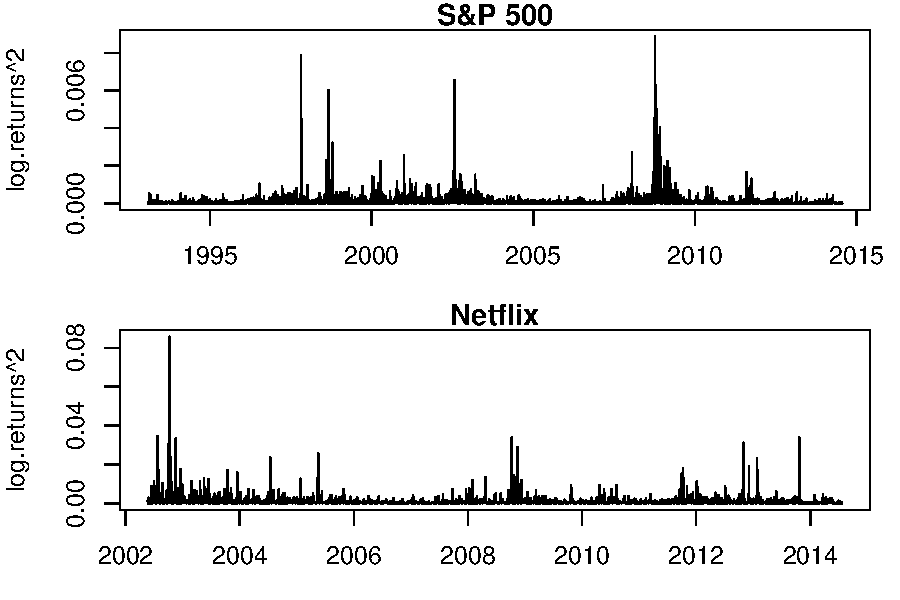
\includegraphics[scale=0.8]{SP500-daily-squared-log-returns.pdf}
%	\caption{Daily squared log returns for the S\&P 500 index and Netflix, Inc. Evident in this figure is the clustering of periods with low and high daily changes in price, demonstrating that asset volatility fluctuates over time.}
%	\label{fig:SP500-daily-squared-log-returns}
%\end{figure}
%
\begin{figure}[htbp]
        \centering
        \begin{subfigure}[t]{0.4\textwidth}
                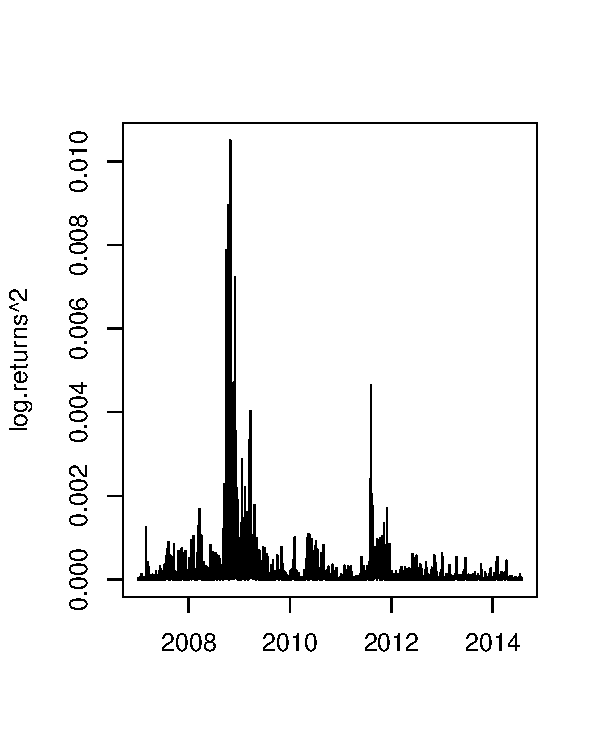
\includegraphics[width=\textwidth]{./chapter-1-introduction/SP500-daily-squared-log-returns.pdf}
                \caption{Daily squared log returns for the S\&P 500 index.}
                \label{fig:sp500-returns}
        \end{subfigure}%
        \quad %add desired spacing between images, e. g. ~, \quad, \qquad, \hfill etc.
          %(or a blank line to force the subfigure onto a new line)
        \begin{subfigure}[t]{0.4\textwidth}
                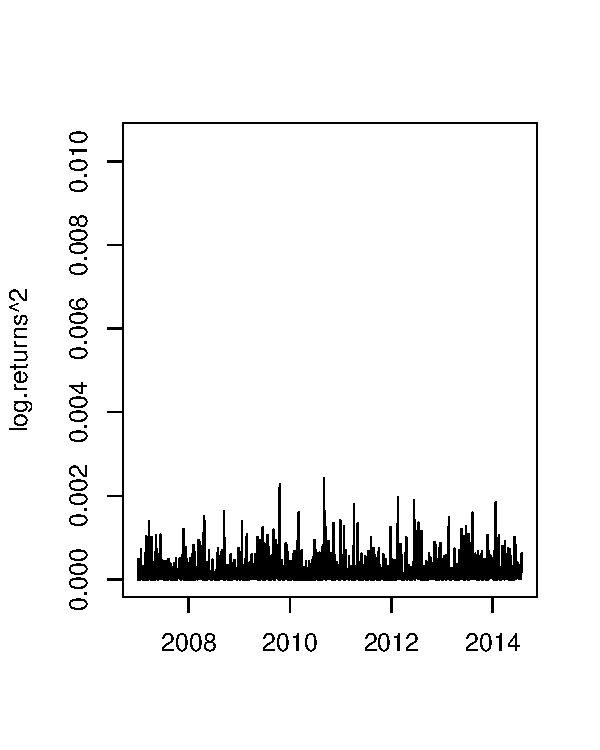
\includegraphics[width=\textwidth]{./chapter-1-introduction/SP500-daily-squared-log-returns-constant-vol.pdf}
                \caption{Simulated daily squared log returns, obtained by sampling a normal distribution with the mean and standard deviation of the S\&P 500 daily log returns. }
                \label{fig:sp500-returns-constant-vol}
        \end{subfigure}
	\\
	\begin{subfigure}[t]{0.4\textwidth}
                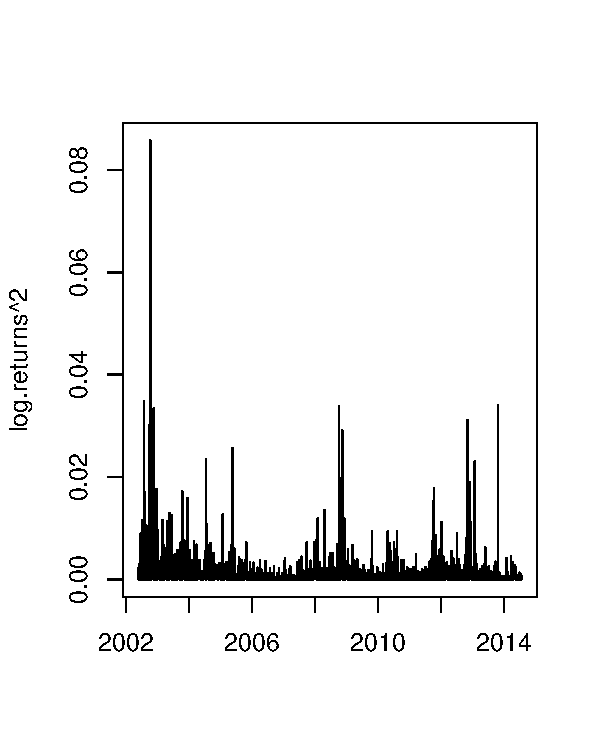
\includegraphics[width=\textwidth]{./chapter-1-introduction/Netflix-daily-squared-log-returns.pdf}
                \caption{Daily squared log returns for Netflix, Inc.}
                \label{fig:netflix-returns}
        \end{subfigure}%
        \quad %add desired spacing between images, e. g. ~, \quad, \qquad, \hfill etc.
          %(or a blank line to force the subfigure onto a new line)
        \begin{subfigure}[t]{0.4\textwidth}
                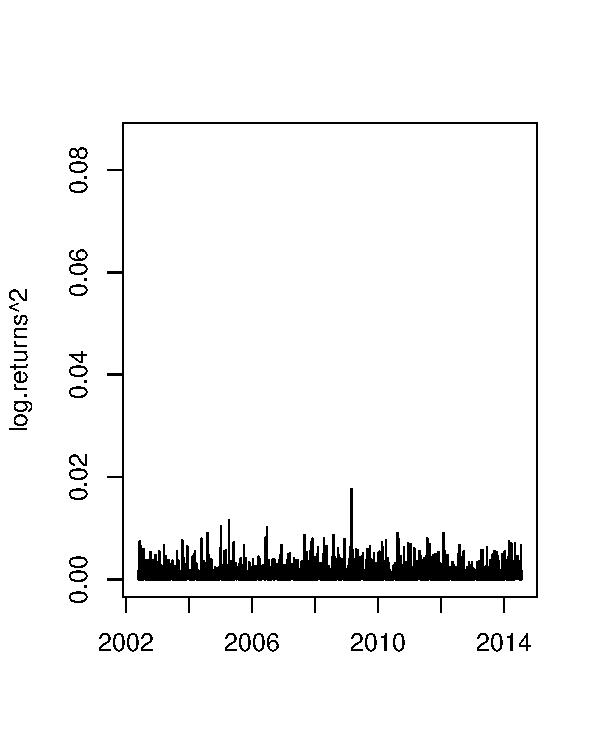
\includegraphics[width=\textwidth]{./chapter-1-introduction/Netflix-daily-squared-log-returns-constant-vol.pdf}
                \caption{Simulated daily squared log returns, obtained by sampling a normal distribution with the mean and standard deviation of the Netflix, Inc. daily log returns. }
                \label{fig:netflix-returns-constant-vol}
        \end{subfigure}
	\caption{Evident in the above figures is the clustering of periods with low and high daily changes in price for the market data, demonstrating that asset volatility fluctuates over time. The constant volatility simulated data is characteristically different from the market data.}
	\label{fig:squared-log-returns}
\end{figure}

\section{Review of Models for Time-varying Volatility}
The literature on volatility as a non-constant process ranges from the early autoregressive 
heteroskedastic (ARCH) model by \cite{engle1982} and the generalized version by \cite{bollerslev1986},
to stochastic volatility models \citep*{hull1987pricing}. Most statistical models 
have used opening and closing prices over the frequency considered for estimation and forecasting.

	\subsection{ARCH/GARCH Models}
	The most important development in modeling volatility changes has been the \textit{autoregressive conditional heteroskedasticity} or ARCH model, introduced by \cite{engle1982}. In results from models of inflation, Engle found that large and small forecast errors occurred in clusters, suggesting a form of heteroskedasticity in which the variance depends on the size of previous fluctuations. 

We will introduce ARCH models with the particular ARCH($p$) model. ARCH models use a conditional structure to model time-varying volatility. Assuming that the log returns $r_t$ follow the linear relationship
\begin{align*}
r_t &= \mu + \epsilon_t, &  t=1,\ldots, T, \\
\epsilon_t &\sim N(0, \sigma_t^2)
\end{align*}
%
where $\mu$ is a mean level that may be dependent on regression and explanatory variables, the ARCH($p$) model characterizes the distribution of the stochastic error by imposing an autocorrelated, time-dependent structure on the variance of the noise term
\begin{eqnarray*}
	\sigma_t^2 &=& \omega + \sum_{i=1}^p \alpha_i \epsilon^2_{t-i}, \\
	\epsilon_t &=& \sigma_t Z_t,
\end{eqnarray*}
where $\omega$ and $\{ \alpha_i \}, i=1,\ldots, p$ are nonnegative constants, and $Z_t \sim N(0,1)$. The conditional variance function is formulated to mimic the phenomenon of large volatility following large shocks to the dependent variable manifested as large deviation of $r_t$ from the mean $\mu$. In other words, high value for $\epsilon_t^2$ increases $\sigma^2_{t+1}$, which in turn increases the expectation of $\epsilon_{t+1}^2$, and so on. 

\cite{bollerslev1986} extended the ARCH($p$) model into the GARCH($p,q$) model, the \textit{generalized} ARCH, by including past variances into the conditional variance formula:

	\[ \sigma_t^2 = \omega + \sum_{i=1}^q \alpha_i \sigma^2_{t-i} + \sum_{i=1}^p \beta_i \epsilon^2_{t-i}. \]
%
This additional feature captures longer-term effects outlasting the impacts of shocks to the dependent variables. One issue is that, if $\alpha_i$ and $\beta_i$ are left unrestricted, the variance can potentially be negative. 

ARCH and GARCH models have been widely successful \citep*{bollerslev2003measuring}, but they fail to capture some important features of financial and economic data. The most important feature not captured is the leverage effect, which has been addressed by Nelson's \textit{exponential} GARCH \citep*{nelson1991conditional} model: 

 	\[ \log \sigma_t^2 = \omega + \sum_{i=1}^p \alpha_i \log \sigma_{t-i}^2 + \sum_{i=1}^q \beta_i g(Z_{t-i}), \]
where 
	\[ g(Z_t) = \theta Z_t + \gamma[ |Z_t| - E|Z_t| ], \] 
with $Z_t \sim N(0,1)$. Assuming that $\gamma > 0$ and $\theta = 0$, the innovations in $\log \sigma^2_{t+1}$ are positive (negative) when the magnitude of $Z_t$ is larger (smaller) than its expected value. If $\gamma = 0$ and $\theta <0$, the innovation in the variance is negative (positive) when $Z_t$ is positive (negative). In this manner the EGARCH model captures the asymmetric leverage effect of negative returns leading to greater volatility, as well as the previously included effect of above (below)-average (in terms of magnitude) residuals leading to greater (smaller) volatility. 

ARCH-type models are appealing because they allow for direct parametric modeling of volatility, and consequentially varieties of models building upon the ARCH, GARCH, and EGARCH models presented so far have been developed. The immediate availability of a conditional likelihood function for the observables allows for standard and efficient MLE methods to be used for fitting \citep*{baillie1991bivariate}, and by an extension, Bayesian analysis is applicable as well \citep{bauwens1998bayesian, nakatsuma2000bayesian, vrontos2000full}. 


	\subsection{Stochastic Volatility}
	Whereas GARCH uses a single stochastic process to drive both the asset and volatility process, stochastic volatility (SV) models are defined by a set of two stochastic differential equations that define separate (but possibly dependent) evolutions for the asset and volatility:
\begin{eqnarray}
	dS_t &=& \mu(S_t, \sigma_t)dt + \nu(S_t, \sigma_t)dW_{t,1} \label{eq:SV-model-1}, \\
	d\sigma_t &=& \alpha(S_t, \sigma_t)dt + \beta(S_t, \sigma_t)dW_{t,2}, \label{eq:SV-model-2}.
\end{eqnarray}

One of the first and most well-known continuous-time SV models was introduced by \cite{hull1987pricing}. In it, the log price follows Brownian motion (so that the price follows GBM) with changing volatility, and the volatility follows an Ornstein-Uhlenbeck (OU) process:
	\begin{eqnarray*}
			d Y_t &=& \mu dt + \sigma_t dW_{t,1} \\
			d \log( \sigma_t ) &=& \alpha(\phi - \log(\sigma_t))dt + \omega dW_{t,2} 
	\end{eqnarray*}

Discretizing the continuous-time model above produces the state-space model
\begin{align*}
	Y_t 			&= \mu + Y_{t-1} + \epsilon_t^1 								 & \epsilon_t^1 \sim N(0, \sigma_t^2), \\
	\log(\sigma_t) &= \alpha + \phi \left[ \log(\sigma_{t-1}) - \alpha \right] + \epsilon_t^2  & \epsilon_t^2 \sim N(0, \tau^2),
\end{align*}
which is the model proposed by \cite{clark1973subordinated}, one of the first papers in which serial correlation is allowed in the volatility process.  

%Expressed in integral form, the standard SV model becomes 
%	\begin{eqnarray}
%		S_t =  S_0 + \int_0^t \mu(S_s, \sigma_s) ds + \int_0^t \nu(S_s, \sigma_s) dB_{s,1} \\
%		\sigma_t = \sigma_0 +  \int_0^t \alpha(S_s, \sigma_s) ds + \int_0^t \beta(S_s, \sigma_s) dB_{s,2}
%	\end{eqnarray}

%	One of the first papers on SV that does allow for serial correlation is by Taylor (1982) who introduced his model in the discrete time setting. The risky part of returns was modeled as the process
%	\[ m_i = M_i - M_{i-1} = \int_{t_i}^{t_{i+1}} \sigma_s dW_s = \sigma_i \epsilon_i. \]
%It was assumed that $\sigma_i$ and $\epsilon_i$ are independent, and that $\epsilon$ has mean zero and unit variance. Hence, $\sigma_i$ can be thought of as the variance of the random process, allowed to vary from timestep to timestep. The change of $\sigma_i$ over timesteps is modeled with autoregressive process
%	\begin{eqnarray*}
%		\sigma_i &=& \exp(h_i/2) \\
%		h_{i+1} &=& \mu + \phi(h_i - \mu) + \nu_i
%	\end{eqnarray*}
%	where $\nu_i$ is Gaussian with zero mean and unit variance. If $\epsilon_i$ is assumed to be Gaussian, this is the log-normal model. The general formulation above allows for direction of returns to influence future volatility by correlating $\epsilon$ and $\nu$. This captures the important empirically observed leverage effect.

%One mathematically tractable and widely used parameterization of the general form of SV models is where the price follows GBM with changing volatility, and the volatility follows an Ornstein-Uhlenbeck (OU) process
%\begin{eqnarray*}
%	dY_t &=& \mu dt + \sigma_t dB_{t,1} \\
%	d\log(\sigma_t) &=& \kappa(\theta - \log(\sigma_t)) + \tau dB_{t,2}.
%\end{eqnarray*}

%One of the first and most well-known continuous-time SV model was introduced by Hull and White \cite{hull1987pricing} in 1987. They proposed two continuous time SV model, the latter one being:
%	\begin{eqnarray*}
%			d \log(Y_t) &=& \mu(Y_t, t) dt + \sigma(Y_t, t) dW_t \\
%			d \log( \sigma^2 ) &=& \alpha(\mu - \log(\sigma^2))dt + \omega dB 
%	\end{eqnarray*}
%where $\omega(\cdot)$ is a non-negative deterministic function and $B$ is a second Brownian motion. Discretization of this model produces the model suggested by Taylor. 

From the late 1990s, stochastic volatility models have taken center stage in econometric analysis of volatility forecasting \citep*{shephard2005selected-readings}. Stochastic volatility models can capture time clustering \citep*{hull1987pricing}, as well as leverage effects \citep*{yu2005leverage} by introducing correlation between $W_{t,1}$ and $W_{t,2}$. 

Empirical evidence suggests that, across different asset types and timescales, the dependence in the volatility structure initially decays quickly at short lags but then decays slowly at longer lags \citep*{andersen1997heterogeneous, andersen1997intraday, andersen1998answering}. For this reason, effort has been placed on developing both continuous and discrete-time long-memory SV models. In the discrete case, one approach has been to model log volatility as a fractionally integrated process \citep*{harvey2002long, breidt1998detection-estimation}. In continuous time, the log volatility has been modeled as fractionally integrated Brownian motion \citep*{comte1998long}, and a square root model driven by fractionally integrated BM \citep*{comte2012affine}. Another important extension includes the addition of jumps in the diffusion of price \citep*{bates1996jumps}. 

Fitting stochastic volatility models is made difficult by the non-linearities of the likelihood as well the large sample space formed by the latent series $\{ \sigma_t \}$. Techniques for estimation of SV models include quasi-maximal likelihood approaches as done by \cite{ruiz1994quasi}, the particle filter approach of \cite{sandmann1998estimation}, the generalized method of moments \citep*{melino1990pricing}, and MCMC methods \citep*{jacquier2002bayesian, kim1998stochastic, omori2007stochastic}.

	\subsection{ Time-changed Brownian Motion}
	A more general approach for representing changing volatility in financial assets, which encompasses both stochastic volatility and GARCH-type models, is time-changed Brownian motion. Time-changed Brownian motion was first used in the paper of \cite{clark1973subordinated}, which introduced the concept into financial economics. Under time-changed Brownian motion, the log-price $Y$ of an asset is written as 
	\begin{equation}
		Y_t = W_{\tau_t}, \quad t \geq 0,
	\end{equation}
	where $W$ is Brownian motion, $t$ is continuous time and $\tau_t$ is a non-negative process with non-decreasing sample paths. If $W$ and $\tau$ are independent, $Y_t | \tau_t \sim N(0, \tau_t)$. In this case, it is immediately obvious that this formulation allows for the second moments of the price process to change over time. Further, marginally $Y_t$ is a scale mixture of normals, which means that returns are symmetric but can be fat tailed. The time-change process $\tau_t$ can be modeled as either a function of some observables, or as a latent process, which is more in line with the modern development of stochastic volatility. 

Time-changed Brownian motion has also become a popular tool for building financial models \citep*{geman2005measure}. Stochastic processes of this kind can capture asset price jumps, changing return volatility, and correlation between volatility and asset returns \citep*{carr2004time}. The mathematical treatment of these models usually involves the computation of the characteristic function, which is typically easy to get as long as $\tau$ and $W$ are independent. However, even if the characteristic function is available in closed form, the associated density often needs to be computed numerically.

%Since the work of Heston \cite{heston1993closed}, focus has been placed on the use of characteristic functions for understanding proposed processes. A closed-form expression for the characteristic function allows for a closed-form expression for the probability density of the underlying asset price. Such a likelihood function can be used to find MLE for model parameters, as well as for evaluating option prices.
%However, Clark's paper did not allow for serial correlation of increments of $\tau_t$ that would generate clustering in $M$. 
%	Putting Clark's paper in a more modern context, as long as $E(\sqrt{\tau_t}) < \infty$, he modeled the ``risky'' part of a semimartingale 
%	\[ Y = A + M, \]
%where the increments of $A$ is the reward component compensating the investor for taking on the risky component $M$. Conditioning on the time-change process $\tau_t$, we have 
%	\[ Y_t | \tau_t \sim N( f(\mu, t, \tau_t), \tau_t), \]
%where $\mu$ is some vector of parameters. We see that this is the more general version of the solution to the stochastic differential equation (\ref{eq:SDE-geo-BM}). 

%	\section{Range-Based Estimation}
%	As we saw in the previous section, realized variance is a ex-poste volatility estimator that can be used to fit continuous (through GMM) and discrete-time (state-space representation) SV models. To improve model fitting and estimation for SV models, we can use the price range within a sampling interval $\Delta$ for an asset, as in \cite{alizadeh2002range}. We denote the range-based statistic as $f(S_{i\Delta}, S_{(i+1)\Delta})$, again where $S_t$ is the price of the asset. If the estimator is homogeneous in the volatility, we write
%\[ f(S_{i\Delta}, S_{(i+1)\Delta}) = \sigma_{i\Delta}^\gamma f(S^*_{i\Delta}, S^*_{(i+1)\Delta}), \]
%where $S^*_t$ is the standarized diffusion. 
%Hence, if the latent volatility follows an OU-process, we can write the state-space model 
%\begin{eqnarray*}
%	\log(\sigma_{(i+1)\Delta}) &=& \alpha + \phi \left[ \log(\sigma_{(i-1)\Delta}) - \alpha \right] + \epsilon_{(i+1)\Delta}\\
%	\log\left| f(S_{i\Delta}, S_{(i+1)\Delta}) \right| &=& \gamma \sigma_{(i+1)\Delta} + E\left( \log\left| f(S^*_{i\Delta}, S^*_{(i+1)\Delta}) \right| \right) + \nu_{(i+1)\Delta},
%\end{eqnarray*}
%where $\sigma_{i\Delta}$ is the assumed constant volatility over $\Delta$. This can be estimated, once more, with a Kalman filter. The usefulness of this approach lies in that we can use different estimators for the volatility $f(S_{i\Delta}, S_{(i+1)\Delta})$, and that the dynamical model form is convenient and efficient to use for both estimation and prediction. 

\section{Time-Varying Volatility in High-Frequency Data}
The advent of electronic trading has allowed for the increase in the volume and speed at which transactions on financial markets are performed and recorded. Today, transactions occur on a microsecond timescale \citep*{brogaard2010high} for certain types of assets, and there has been increasing interest in using this data to better understand volatility in financial markets. 

Much of the effort to use high-frequency data to understand the evolution of volatility has focused on \textit{realized volatility}. The concept of realized volatility was introduced in three independent papers by \cite{andersen2001distribution}, \cite{barndorff2002estimating}, and \cite{comte1998long} as a means to perform the estimation of $\int_t^{t+\Delta} \sigma^2(Y_s, s) ds$, where $\Delta$ is some finite period of time and $y_t$ is the log-price of the asset following a diffusion process. 

Let $\Delta = 1$ day, and suppose there are $m$ observation of the price over the trading period. The $i^{th}$ interday log-return is defined as 
\begin{align*}
r_i^{(m)} &= y_{i/m} - y_{(i-1)/m}, &  i =1, \ldots, m.
\end{align*}

The sum of the squared log intraday returns is the realized volatility
\begin{equation}
	RV^{(m)} = \sum_{i=1}^m r_i^{(m)^2}. \label{eq:RV}
\end{equation}
It can be shown that $RV^{(m)} \xrightarrow{p} \int_t^{t+\Delta} \sigma^2(Y_s, s)ds$ as $m \to \infty$. Realized volatility is a consistent estimator of the integrated volatility \citep*{barndorff2002econometric}, and it is asymptotically distributed:
\begin{equation}
 \frac{\sqrt{m} (RV^{(m)} - \int_{t}^{t+\Delta} \sigma^2(Y_s,s)ds)}{\sqrt{ 2\int_{t}^{t+\Delta} \sigma^4(Y_s,s)ds} } \xrightarrow{d} N(0,1) \label{eq:asy}
\end{equation}

\cite{barndorff2004power} also propose a consistent estimator for the power variation $\int_{t}^{t+\Delta} \sigma^4(y_s,s)ds$, which is needed to construct credible confidence intervals given the result in equation (\ref{eq:asy}). There has been further work in the derivation of consistent estimators of higher moments of the integrated volatility, which are used in the estimation of continuous time SV models with higher frequency data \citep*{todorov2011econometric}.

%The realized volatility estimator is a nonparametric estimator with very desirable asymptotic properties, given that the assumptions on the diffusion process for the log-price hold. Yet one problem with using RV alone is that it can only estimate the integrated volatility over $\Delta$. In other words, practitioners can use RV as a stand-alone tool to at best estimate the average of the volatility process over the sampling period. 

	\subsection{Microstructure Noise}
One challenge with the analysis of high-frequency price data is the presence of microstructure noise at the microsecond timescale. As the sampling period shrinks down to the transaction-by-transaction frequency, irregular spacing between transactions, discreteness in transaction prices, and very short-term temporal dependence become dominant features of the data \citep*{stoll2000presidential}. For this reason, the foundational diffusion assumption on the log-price of assets no longer holds. Measurements at high frequencies no longer capture only the evolution of prices, but they capture a noisy version of the price. 

In the model-free setting of realized volatility estimators, one approach to mitigating the confounding effects of microstructure noise is to combine averaged RV estimates obtained by subsampling the data with a RV estimate using all available data \citep{zhang2005tale}. Another approach is to employ a class of kernel-based methods similar to those used for estimating the long-run variance of a stationary time-series in the presence of autocorrelation \citep{hansen2006realized}. 

In the context of stochastic volatility, microstructure noise could, for example, be accounted for with a model of the form:
\begin{eqnarray*}
	Y_{t+1} &=& \log(S_{t+1}) + m_{t} \\
	\log(S_{t+1}) &=& \log(S_{t}) + \mu(S_t, \sigma_t) + \nu(S_t, \sigma_t)\epsilon_{t+1,1} \\
	\log(\sigma_{t+1}) &=& \log(\sigma_{t}) + \alpha(S_t, \sigma_t) + \beta(S_t, \sigma_t)\epsilon_{t+1,2}.
\end{eqnarray*} 
The distributional assumptions on the noise $m_t$ can be varied, and there can be correlation between the innovation terms $\epsilon_{t+1,1}$ and $\epsilon_{t+1,2}$
%
%For the above-mentioned reasons, the realized volatility estimator is often used as part of an inferential model.

	\subsection{Stochastic Volatility Models and High-frequency Data} \label{sec:stoch-vol-models-and-high-freq-data}
One of the first papers to use realized volatility in the estimation of continuous-time SV models is by \cite{barndorff2002econometric}. The idea of the paper is use the continuous time SV model and the RV estimator to form a state-space model, which can be estimated with a Kalman filter.

Assuming the variance $\sigma^2(t)$ follows the Ornstein-Uhlenbeck (OU) process instead of the log-variance, the autocorrelation function for the volatility is known to be $r(t, t') = \exp(-\lambda \left| t' - t \right|)$. The functional form for $r(t)$ allows for the explicit form of the correlation function between observations in the volatility process:
%
\[ corr(\sigma^2_{t}, \sigma^2_{t+s}) = d \exp(t\{ -\lambda\Delta(s-1) \}), \]
%
where $d$ is a constant in terms of $\lambda$ which is less than 1, and $\Delta$ is the length of time between returns. Hence, the actual volatility has the autocorrelation function of an autoregressive moving average (ARMA) model of order (1,1). Letting $RV^{(m)}_t$ be the realized volatility in interval $(t-\Delta, t)$ computed with $m$ intraperiod observations, $RV^{(m)}_t$ can be decomposed in terms of the true volatility for the interval plus an error term $u_t$ due to microstructure noise
\begin{equation}
	RV^{(m)}_t = \sigma^2_t + u_t. \label{eq:decomposition}
\end{equation}
Setting $E(\sigma^2_t) = \xi \Delta$, and using the ARMA(1,1) representation of the volatility process, equation (\ref{eq:decomposition}) becomes
\[
	RV^{(m)}_t = (\xi \Delta + \phi \sigma^2_{t-1} + \theta \sigma_{\sigma}\epsilon_{t-1} + \sigma_{\sigma}\epsilon_{t} ) + (\sigma_u \nu_t),
 \]
where $\epsilon_{t-1}, \epsilon_t, \nu_t \sim N(0,1)$. The parameter $\sigma_{\sigma}$ is the standard deviation of the innovations driving the volatility process, $\sigma_u$ is the standard deviation of the microstructure noise, and $(\phi,\theta)$ are the ARMA parameters. Therefore, the realized volatility observations can be expressed as the state-space model
\begin{eqnarray*}
	RV^{(M)}_t &=& \Delta \xi + (1 \quad 0 )\alpha_t + \sigma_u v_{t} \\
	\alpha_{t} &=& \left( \begin{array}{cc} \phi & 1 \\ 0 & 0 \end{array} \right) \alpha_{t-1} + \left( \begin{array}{c} \sigma_\sigma \\ \sigma_\sigma \theta \end{array} \right) \epsilon_{t},
\end{eqnarray*}
which can be estimated with a Kalman filter.

An alternative approach for estimating SV models using realized volatility data is based on the generalized method of moments. In this method, higher powers of realized volatility are used as approximations to higher orders of integrated volatility, as done by \cite{bollerslev2002estimating}. By matching the sample moments of the realized volatility to the moments of the integrated volatility implied by the continuous-time SV model, a generalized method of moments estimator for the underlying model parameters can be obtained. Some more recent works dealing with fitting stochastic volatility models to high-frequency data include that of \cite{venter2012extended} and \cite{shirota2014realized}.

\section{Plan for the Advancement}
In Chapter \ref{chapter:2} we will derive the likelihood for closing prices of financial asset prices that takes into account the highest and lowest prices within a trading period. We also compare maximum likelihood estimates for volatility based on this approach to realized volatility estimates using simulated high-frequency data. In Chapter \ref{chapter:3} we extend the model in Chapter \ref{chapter:2} to two dimensions and examine the convergence properties of the thus-derived likelihood solution. In Chapter \ref{chapter:4} we outline the future direction of this project. 

%In the general setting of (\ref{eq:SV-model-1}) - (\ref{eq:SV-model-2}), the estimation of volatility parameters based on the discretely sampled observations is complicated by the $\sigma(t)$ process being latent. However, as already discussed, realized volatility approximates almost surely $\int_t^T \sigma^2(s)ds$ as the sampling frequency increases. Hence, explicitly treating the integrated volatility as observable allows the implementation of generalized method of moments-like estimators. 

%Considering the model 
%\begin{eqnarray}
%	dY_t &=& \sqrt{V_t}dB_t \\
%	dV_t &=& \kappa(\theta - V_t)dt + \sigma\sqrt{V_t}dW_t, 
%\end{eqnarray}
%the authors develop the conditional expectations for the integrated volatility $\int_{t+1}^{t+2} V_s ds$ and integrated variance $\int_{t+1}^{t+2} V^2_s ds$, given a filtration $G_t$ up to time $t$:
%\begin{eqnarray*}
%	E\left( \int_{t+1}^{t+2} V_s ds | G_t \right) &=& \alpha E\left( \int_{t}^{t+1} V_s ds | G_t \right) + \beta, \\
%	E\left( \int_{t+1}^{t+2} V^2_s ds | G_t \right) &=& H E\left( \int_{t}^{t+1} V^2_s ds | G_t \right) + I E\left( \int_{t}^{t+1} V_s ds | G_t \right) + J,
%\end{eqnarray*}
%with $H, I$, and $J$ being defined in terms of the model parameters. The analytical solutions for the conditional first and second moments allow for the construction of a standard GMM estimator for the model parameters. 

%	\subsection*{Non-equally spaced observations}
%	Financial transaction data inherently arrive in irregular time intervals in the form of bid and ask offers of market traders. Frequently traded stocks will have transactions every few seconds, while commodities will have transactions every day or even every week. If a short interval is chosen for econometric analysis, there will be many intervals with no new information and heteroskedasticity will be introduced into the data, yet if a lzonger interval is chosen multiple  transactions will be averaged and potential covariate relationships in the data will be lost, thereby making high-frequency data not extra advantageous. What complicates the choice of a best time intervals for econometric analysis is that the rate of transaction arrival within any chosen fixed interval may vary over its course, and also that any asset traded may randomly exhibit unusual activity due to an unobservable event (with respect to the asset price). 

%	An alternative to fixed interval analysis is proposed in \cite{engle1998autoregressive} with the autoregressive conditional duration model (ACD). The arrival times of market events, such as price changes and volume of trade offers, are represented as random variables following a self-exciting point process, where the means of arrival time intervals are modeled as an ARMA process. Each arrival interval is then represented by its expected duration times an innovation term, which in this paper is the Weibull distribution. The intensity of arrivals is a baseline function multiplied by a normalized current time interval with respect to the conditional expected duration. The baseline intensity is modeled semi-parametrically and inter-day trading effects are included. The model is used to estimate and forecast the intensity of transaction arrivals and hence get an estimate of instantaneous volatility, as well as test hypotheses about market microstructure. This model is used in \cite{russell1998}, where additionally conditional, discrete price transition probabilities are developed. 

%	Their approach has been subsequently extended by many authors. Bauwens and Giot [3] put forth a log-linear specification for the conditional mean which always guarantees the positivity of the durations without imposing restrictions on the coefficients. Zhang et al. [25] introduced a non-linear version of the ACD model in the spirit of the linear autoregressive threshold models. Bauwens and Veredas [5] proposed a stochastic duration model which is analogous to the stochastic volatility models in the same way as the Engle and Russel’s ACD model is analogous to the GARCH model. Ghysels et al. [14] considered a rather complicated version of the ACD model, which allows disentangling the dynamics of the mean and the variance of the duration process. In addition to the exponential and Weibull distributions for the error terms, other distributions have been proposed. Grammig and Maurer [16], and Grammig and Wellner [17] consider the Burr distribution and Lunde [20] considers the generalized gamma distribution. The log-normal distribution, although seemingly a natural candidate, has received limited attention in the literature with the exception of the work by Allen et al. [2] and Sun et al. [24]. Despite this impressive body of work, only a limited number of papers have been devoted to testing the specifications of the alternative ACD models. Two notable exceptions are the work of Fernandes and Grammig [13] and Bauwens et al. [4]. The first paper evaluates ACD models by gauging the distance between the parametric density of the duration process and its non-parametric estimate, using the methods developed by Ajt-Sahalia1 [1]. Only the standard ACD specification of Engle and Russel1 [11] is considered, using error terms with exponential,Weibull, generalized gamma and Burr distributions. Employing only one sample of durations for Exxon, these authors find that the Burr and generalized gamma distributions perform better than the exponential and Weibull distributions. Bauwens et al. [4], using the methodology for evaluating density forecasts by Diebold et al. [9], consider a number of alternative ACD specifications for three stocks traded on New York stock exchange. One of their main findings is that the exponential and Weibull distributions are often mis-specified, while on the other hand Burr and generalized gamma distributions perform much better. Additionally, they find that the specification for the conditional mean (e.g. the standard ACD, log-ACD as well as non-linear approaches such as the Threshold ACD model) does not seem to affect the models’ performance much. In particular, their results suggest very little difference between the ACD and log-ACD specifications.


%We also aim use the range of the asset price over $\Delta$, but by formally incorporating the information within the likelihood model that is given by assumption that log-price, $Y_t$, follows a diffusion process. Assuming that $\sigma$ is constant over the period of interest, the log-price follows the SDE
%\begin{equation}
%	dY_t = \mu dt + \sigma dW_t, \label{eq:SDE}.
%\end{equation}
%Using the Fokker-Planck Equation, we can take the SDE in (\ref{eq:SDE}) and express the probability density of the asset price $f(y,t)$ as the PDE
%\begin{eqnarray*}
%	\frac{\partial}{\partial t} f(y,t) &=& -\mu \frac{\partial}{\partial y}f(y,t) + \frac{1}{2}\sigma^2 \frac{\partial^2}{\partial y^2} f(y,t), \\
%	f(y,0) &=& \delta(y-y_0),
%\end{eqnarray*}
%where $y_0$ is the price at the beginning of the interval.
%The function $f(y,t)$ is the probability that $Y_t = y$, namely that the log-price of the asset is $y$ at time $t$. Without any additional restrictions, therefore, for any time period $\Delta$, we have the likelihood of a closing price, given the parameters $\mu$ and $\sigma$. Now, we incorporate the information that, for the observed path of the process, $\max\left\{ y \right\} = A$ and $\min\left\{ y \right\} = a$. Since $f(y,t)$ is the probability distribution of the price at time $t$, and $y(t)$ is the realization of the underlying stochastic process, in just the same way $A$ and $a$ are the realizations of the maximum and mininum of the process up to time $t$.  Hence, we can impose the condition that the maximum of the process $\sup\left\{ Y_t \right\}$ must, in general, be below $A$ and the minimum of the process $\inf\left\{ Y_t \right\}$ must exceed $a$. With the max/min information, the diffusion process SDE is modified to 
%\begin{equation}
%	dY_t = \mu dt + \sigma dW_t, \qquad \sup\left\{ Y_t \right\} \leq A \quad \inf\left\{ Y_t \right\} \geq a.
%\end{equation}
%In terms of the probability density, the SDE is now
%\begin{eqnarray}
%	\frac{\partial}{\partial t} f(y,t) &=& -\mu \frac{\partial}{\partial y}f(y,t) + \frac{1}{2}\sigma^2 \frac{\partial^2}{\partial y^2} f(y,t) \label{eq:IC-BV-1}\\
%	f(y,t) \leq A && f(y,t) \geq a, \qquad f(y,0) = \delta(y-y_0). \label{eq:IC-BV-2}
%\end{eqnarray}
%The solution to the IC/BV problem is interpreted as 
%\[ f(y,t) = P( \inf\{Y_t\} \geq a, \sup\{Y_t\} \leq A, Y_t = y | Y_0 = y_0 ). \]
%Thus, 
%\[ -\frac{\partial^2}{\partial A \partial a} f(y,t) = P( \inf\{Y_t\} = a, \sup\{Y_t\} = A, Y_t = y | Y_0 = y_0 ). \]
%The probability density function above is very important, as its maximization over the parameters $\mu$ and $\sigma$ produces maximum likelihood estimates $\hat{\mu}$ and $\hat{\sigma}$, which incorporate the max/min information over the period $\Delta$. MLE estimates are consistent and efficient, so that the estimators based on the solution to the IC/BV problem above will outperform other ad-hoc range-based estimators.

%\subsection*{Solution to the IC/BV Problem}
%The solution to the problem in (\ref{eq:IC-BV-1}) - (\ref{eq:IC-BV-2}) begins with a change of coordinates which transforms the advection-diffusion problem to a purely diffusion problem. Let 
%\[ f(y,t)=  \exp(ay + bt)u(y,t), \]
%so that 
%\begin{eqnarray*}
%	\frac{\partial}{\partial t} f(y,t) &=& -\mu \frac{\partial}{\partial y} (\exp(ay + bt) u(y,t)) + \frac{1}{2}\sigma^2\frac{\partial^2}{\partial y^2} (\exp(ay + bt) u(y,t)) \\
%		&= & -\mu \left[ a \exp(ay + bt) u(y,t) + \exp(ay + bt) \frac{\partial}{\partial y} u(y,t)  \right] \\
%		&& + \frac{1}{2}\sigma^2 \left[ a^2 \exp(ay + bt) u(y,t) + a \exp(ay + bt) \frac{\partial}{\partial y} u(y,t) + \exp(ay + bt) \frac{\partial^2}{\partial y^2} u(y,t) \right] \\
%		&=& u(y,t)\left[ -\mu a + \frac{1}{2}\sigma^2 a^2 \right] \exp(ay+bt) \\
%		&& + \frac{\partial}{\partial y} u(y,t)\left[ -\mu + \frac{1}{2}\sigma^2 a \right]\exp(ay+bt) \\
%		&& + \frac{\partial^2}{\partial y^2} u(y,t) \left[ \frac{1}{2}\sigma^2 \right] \exp(ay+bt) \\
%		&=& b\exp(ay+bt)u(y,t) + \exp(ay+bt)\frac{\partial}{\partial t}u(y,t) 
%\end{eqnarray*}

%We thus have the condition
%\begin{equation}
%	u(y,t)\left[ -\mu a + \frac{1}{2}\sigma^2 a^2 \right] + \frac{\partial}{\partial y} u(y,t)\left[ -\mu + \frac{1}{2}\sigma^2 a \right] + \frac{\partial^2}{\partial y^2} u(y,t) \left[ \frac{1}{2}\sigma^2 \right] = bu(y,t) + \frac{\partial}{\partial t}u(y,t) 
%\end{equation}
%The system 
%\begin{eqnarray*}
%	-\mu a + \frac{1}{2}\sigma^2 a^2 &=& 0 \\
%	b &=& 0
%\end{eqnarray*}
%defines $a = \sqrt{2\mu}/\sigma$, and $b=0$ such that the original problem is reduced to the heat equation on a bounded domain, with the same IC/BV conditions:
%\begin{eqnarray*} 
%\frac{\partial}{\partial t}u(y,t) &=& \frac{1}{2}\sigma^2 \frac{\partial^2}{\partial y^2} u(y,t) \\
%					u(y,t) &=& 0, \quad \mbox{for} \quad y = a, A \\
%					u(y,0) &=& \delta(y-y_0)
%\end{eqnarray*}

%We can solve the given problem with a Fourier-series representation of the solution:

%\begin{equation} 
%	u(y,t) = \sum_{n=1}^\infty a_n(t)\sin\left( \frac{n \pi (y+a)}{L_y} \right), \quad L_y = A-a \label{eq:trig-exp}
%\end{equation}

%We choose the collection of the odd trigonometric functions as a basis for the solution because they preserve the boundary conditions under the spatial differential operator, and they form a complete basis for solutions to the PDE. 
%Substituting (\ref{eq:trig-exp}) into the PDE produces a differential equation of the time-dependent coefficients:
%\[
%	\dot{a}_n(t)\sin\left( \frac{n \pi (y+a)}{L_y} \right) = - \left( \frac{n\pi}{L_y} \right)^2 a_n(t)\sin\left( \frac{n \pi (y+a)}{L_y} \right)
%\]
%Therefore, the expression for the coefficients is 
%\begin{equation}
%	a_n(t) = a_{n,0} \exp\left( - \left( \frac{n\pi}{L_y} \right)^2 t \right) ,
%\end{equation}
%where $a_{n,0}$ is the coefficient for the sine series representation of the initial condition $\delta(y-y_0)$. Having obtained the solution, we can take derivatives with respect to the max and min values $a, A$ in order to obtain an expression for the likelihood. 

\chapter{Range-Based Methods for High-Frequency Data} \label{chapter:2}

Wider availability of tick-by-tick/bid-ask financial transaction data has motivated the development of models that utilize this information to better estimate asset volatility. We focus on an approach which collapses high-frequency intraperiod transaction information in the form of recorded maximum and minimum prices. Work in this direction includes that of \cite{alizadeh2002range}, which uses only the range of an asset over a sampling period to extract latent stochastic volatility, while \cite{lildholdt2002estimation} uses open, high, low, and close data to do maximum likelihood estimation in a GARCH framework. \cite{rodriguez2012} combine the use of open, high, low, and close data with a Bayesian approach to estimation and prediction in a stochastic volatility framework. 
%Realized volatility demands the use of all intraperiod returns to estimate volatility. High-frequency data might not be available (due to data access), and even if available, for short periods, intraperiod returns are affected by mictrostructure noise. For short periods there might also be multiple subsequent observations recording no change in price levels. For these reasons, we are seeking an alternative estimator of volatility with high-frequency data.

\section{Problem Formulation}
Following the approach of \cite{rodriguez2012}, we are interested in finding the joint probability density for the closing, maximum, and minimum prices for an asset during a nominal period $(t-1, t)$. 
%Similarly to \cite{alizadeh2002range}, we use the range of the asset price over a trading period $\Delta$ to better estimate the volatility of the diffusion process. However, instead of just using the range of the price, we also use the opening and closing price over the interval of interest. We can let $\Delta = 1$ nominally, so that the proceeding model is defined on a period $(t-1, t)$. 
Recall the GBM model discussed in Section \ref{section:GBM}. Assuming that $\sigma$ and $\mu$ are constant over the period of interest, the log-price follows the SDE
\begin{equation}
	dY_s = \mu ds + \sigma dW_s, \label{eq:SDE}.
\end{equation}

Using the Fokker-Planck Equation, we can take the SDE in (\ref{eq:SDE}) and express the probability density of the asset price $q(y,s)$ as the PDE
\begin{eqnarray}
	\frac{\partial}{\partial s} q(y,s) &=& -\mu \frac{\partial}{\partial y}q(y,s) + \frac{1}{2}\sigma^2 \frac{\partial^2}{\partial y^2} q(y,s),  \label{eq:IV-1} \\
	q(y,t-1) &=& \delta(y-y_{t-1}), \label{eq:IV-2}
\end{eqnarray}
where $y_{t-1}$ is the price at the beginning of the interval and $\delta$ is the Dirac delta function.

The value $q(y,t)$ is the probability that $Y_t = y$, namely that the log-price of the asset is $y$ at the end of the time interval. Without any additional restrictions, therefore, the solution to the initial value problem (\ref{eq:IV-1}) - (\ref{eq:IV-2}) constitutes the likelihood of a closing price, given the parameters $\mu$ and $\sigma$, at time $s$.

Now we can incorporate the information for the high and low prices within our model if we restrict the stochastic process so it does not go below or above a certain range:
\begin{eqnarray}
	dY_s &=& \mu ds + \sigma dW_s, \label{eq:SDE-bc-1} \\
	a_t < &Y_s& < b_t. \label{eq:SDE-bc-2}
\end{eqnarray}
Equivalently, we can consider the initial value/boundary condition problem, where the boundary conditions correspond to the process having zero probability of going beyond $a_t$ and $b_t$:
\begin{eqnarray}
	\frac{\partial}{\partial s} q(y,s) &=& -\mu \frac{\partial}{\partial y}q(y,s) + \frac{1}{2}\sigma^2 \frac{\partial^2}{\partial y^2} q(y,s),  \label{eq:IV-BC-1} \\
	q(y,t-1) &=& \delta(y-y_{t-1}), \label{eq:IV-BC-2} \\
	q(a_t,s) = 0, && q(b_t, s) = 0. \label{eq:IV-BC-3} 
\end{eqnarray}

The problem in (\ref{eq:IV-BC-1}) - (\ref{eq:IV-BC-3}) can be further simplified by a transformation which eliminates the first derivative term, thereby transforming the advection-diffusion problem to a purely diffusion problem. Letting 
\begin{equation}
	q(y,s) = \exp(ay + bs)p(y,s), \label{eq:q}
\end{equation}
we apply the spatial differential operator and the time-derivative to the right side of equation (\ref{eq:q}) and equate the two expressions. We thus obtain the differential equation

\begin{equation}
 p(y,s)\left[ -\mu a + \frac{1}{2}\sigma^2 a^2 \right] + \frac{\partial}{\partial y} p(y,s)\left[ -\mu + \frac{1}{2}\sigma^2 a \right] + \frac{\partial^2}{\partial y^2} p(y,s) \left[ \frac{1}{2}\sigma^2 \right] = bp(y,s) + \frac{\partial}{\partial s}p(y,s) 
\end{equation}

The system 
\begin{eqnarray}
	-\mu a + \frac{1}{2}\sigma^2 a^2 &=& 0 \label{eq:a} \\
	b &=& 0 \label{eq:b}
\end{eqnarray}
defines $a = \sqrt{2\mu}/\sigma$, and $b=0$ such that the original problem is reduced to the heat equation on a bounded domain, with the same IC/BV conditions:
\begin{eqnarray} 
\frac{\partial}{\partial s}p(y,s) &=& \frac{1}{2}\sigma^2 \frac{\partial^2}{\partial y^2} p(y,s)  \label{eq:heat1} \\
					p(y,s) &=& 0, \qquad \qquad \quad \mbox{for}  \quad y = a_t, b_t \label{eq:heat2} \\
					p(y,0) &=& \delta(y-y_{t-1})  \label{eq:heat3}
\end{eqnarray}

%Letting $M_t = \sup_{s \in (t-1,t)}\{ Y_s \}$ and $m_t = \inf_{s \in (t-1,t)}\{ Y_s \}$, the solution to the IV/BV problem is the probability  
%\[ q(y,t) = P( m_t \geq a_t, M_t \leq b_t, Y_t = y | Y_{t-1} = y_{t-1}, m_t < M_t ). \]

%In further using this likelihood for variance estimation, we will assume that the true minimum and maximum prices over the period $(t-1, t)$ are the observed minimum and maximum prices and set them to $a_t$ and $b_t$, respectively. There are two problems with this assumption. First, even under a high frequency sampling, the prices are observed discretely so that the true maximum price is greater than $b_t$ and the true minimum price is less than $a_t$. Second, as sampling frequency increases, microstructure noise becomes more prominent. These two problems will be disentangled later. 

%The above probability is a cumulative density with respect to the boundary values. Hence, the probability density function for the boundary values and closing price is obtained by differentiating twice with respect to $a_t$ and $b_t$
%\begin{equation}
 %-\frac{\partial^2 }{\partial a_t \partial b_t } q(y,t) = P( m_t = a_t, M_t = b_t, Y_t = y | Y_{t-1} = y_{t-1}, m_t < M_t )  \label{eq:likelihood}
%\end{equation}

%This PDF is very important, as its maximization over the parameters $\mu$ and $\sigma$ produces maximum likelihood estimates $\hat{\mu}$ and $\hat{\sigma}$, which incorporate the max/min information over the period $(t-1, t)$. MLE estimates are consistent and efficient, so that the estimators based on the solution to the IV/BV problem will outperform other ad-hoc range-based estimators in the presence of more data. The current approach to estimating volatility, if microsctructure noise is temporarily ignored, is suitable for high-frequency data, because the observed maximum and minimum over a given period approach the true extrema of the prices as sampling frequency increases. 

\subsection{Closed-Form Solution to the IV/BV Problem via Fourier Expansion}

The Strum-Liouville problem in (\ref{eq:heat1}) - (\ref{eq:heat3}) can be solved by recognizing that the solution is separable. By treating the temporal and spatial differential equations independently, the solution to the problem takes on the familiar Fourier series expansion, except the coefficients of the trigonometric terms decay with time
\begin{equation}
	p(y,s) = \sum_{n=1}^\infty C_{n} \exp\left( -\lambda_n s \right) \sin\left( \frac{n\pi (y- a_t)}{b_t - a_t} \right). \label{eq:trig-expansion}
\end{equation}
There are no cosine terms in the expansion as they do not satisfy the boundary conditions. The expression for $\lambda_n$ is found by substituting the solution into the governing system of equations (\ref{eq:heat1}) - (\ref{eq:heat3}) and, after cancellation, 
\[
	\lambda_n = -\frac{1}{2}\sigma^2 \frac{n^2 \pi^2}{(b_t - a_t)^2}
\]

The coefficients $\left\{ C_n \right\}_{n=1}^\infty$ are found by first recognizing an important property of the sine-series expansion of the solution, the orthogonality of the basis functions with respect to an inner product. Defining $\xi = y - a_t$ and $L = b_t - a_t$, the inner product of two functions $h(\xi)$ and $g(\xi)$ is given by $\int_{0}^L h(\xi)g(\xi) d\xi$. The orthogonality is demonstrated by the inner product of two basis functions:
\[
	\int_0^L \sin\left( \xi \frac{n\pi}{L} \right) \sin\left( \xi \frac{m\pi}{L} \right) d\xi =\frac{1}{2} \int_0^L \cos\left( \xi \frac{(n-m)\pi}{L} \right) - \cos\left( \xi \frac{(n+m)\pi}{L} \right) d\xi = \left\{ \begin{array}{cc}
														0 & \mbox{ if } n \neq m \\
														L/2 & \mbox{ if } n = m
													\end{array}
													\right.
\]
Next, we consider the initial condition with $s=0$
\[ p(\xi,0) = \sum_{n=1}^\infty C_n \sin\left( \xi \frac{n\pi}{L} \right) = \delta(\xi - (y_{t-1}-a_t) ). \]
Using the orthogonality condition,
\[
	 \int_0^L p(\xi,0) \sin\left( \xi \frac{n' \pi}{L} \right) d\xi = \sum_{n=1}^\infty C_n \int_0^L \sin\left( \xi \frac{n' \pi}{L} \right) \sin\left( \xi \frac{n \pi}{L} \right) d\xi  = C_{n'} \frac{L}{2}.
\]
Substituting the initial condition,
\[
	\int_0^L p(\xi,0) \sin\left( \xi \frac{n' \pi}{L} \right) d\xi = \int_0^L \delta(\xi - (y_{t-1} - a_t)) \sin\left( \xi \frac{n' \pi}{L} \right) d\xi = \sin\left( (y_{t-1} - a_t) \frac{n' \pi}{L} \right)
\]
From the two conditions, we have a form for the coefficients:
\begin{equation}
	C_{n'} = \frac{2}{L} \sin\left( (y_{t-1} - a_t) \frac{n' \pi}{L} \right)
\end{equation}
Thus, the final form for $p$ is 
\begin{equation}
	p(y,s) = \sum_{n=1}^\infty \frac{2}{L} \sin\left( (y_{t-1} - a_t) \frac{n \pi}{L} \right) \exp\left( -\frac{1}{2}\sigma^2 \frac{n^2 \pi^2}{L^2} s \right) \sin\left( (y-a_t) \frac{n\pi}{L} \right) \label{eq:p}
\end{equation}

Combining equations (\ref{eq:q}), (\ref{eq:a})-(\ref{eq:b}), and (\ref{eq:p}), final solution to the IV/BC problem is
\begin{equation}
	q(y,s) = \exp\left( \frac{\sqrt{2\mu}}{\sigma} y \right) \sum_{n=1}^\infty \frac{2}{L} \sin\left( (y_{t-1} - a_t) \frac{n \pi}{L} \right) \exp\left( -\frac{1}{2}\sigma^2 \frac{n^2 \pi^2}{L^2} s \right) \sin\left( (y-a_t) \frac{n\pi}{L} \right) \label{eq:q-final}
\end{equation}

\subsection{Closed-Form Solution to the IC/BV Problem via Method of Images}
An alternative way to solve the diffusion problem in equations (\ref{eq:heat1}) - (\ref{eq:heat3}) is through the Method of Images. The general idea of the method is to find the fundamental solution to the IC problem in equations (\ref{eq:heat1}) and (\ref{eq:heat3}). For convenience of mathematical notation, we study time evolution from $t$ to $t+1$. The initial value is then $y(0) = y_t$. We enforce the boundary conditions through an appropriate series of reflections. This solution can also be derived probabilistically through the reflection principle for Brownian motion, as given by \cite{freedman1971brownian}.

The solution to the initial condition problem in equations (\ref{eq:heat1}) and (\ref{eq:heat3}) is the Green's function for the heat equation, which is known to be pdf of the Normal distribution with mean $y_{t-1}$ and standard deviation $\sigma \sqrt{s}$:
\begin{equation}
	g_0(y,s) = \frac{1}{\sqrt{2\pi s \sigma^2}} \exp\left( -\frac{1}{2} \frac{(y-y_t)^2}{s\sigma^2} \right) \equiv N(y; y_t, s\sigma^2) \label{eq:fundamental-solution}
\end{equation}

A single \textit{reflection} of the fundamental solution about the boundary point $a_t$ is defined in terms of a translation of the mean $\zeta(y) = 2a_t - y$ (since the fundamental solution is symmetric around the mean) and a negation of the function value, as shown in Figure (\ref{fig:g1}). The resultant reflection, denoted $r_0(y,s)$, satisfies the heat equation in (\ref{eq:heat1}):

\[ r_0(y,s) = -\frac{1}{\sqrt{2\pi s \sigma^2}} \exp\left( -\frac{1}{2} \frac{( y-\zeta(y_t) )^2}{s\sigma^2} \right) = -N(y; \zeta(y_t), s\sigma^2) \]

By construction, both $r_0$ and $g_0$ have the same magnitudes at $y = a_t$ but with opposing signs. The sum of the fundamental solution and its reflection, denoted as $g_1(y,s)$ and shown below in (\ref{eq:sum1}), therefore satisfies the heat equation, as well as  the boundary condition $g_1(a_t, s) = 0$. However, $g_1(y,s)$ does not necessarily satisfy the boundary condition $g_1(b_t, s) = 0$, as illustrated in Figure (\ref{fig:g1}).
%
\begin{equation} 
g_1(y,s) = g_0(y,s) + r_0(y,s) = N(y; y_t, s\sigma^2) - N(y; \zeta(y_t), s\sigma^2) \label{eq:sum1}
\end{equation}
%

%\begin{figure}
%	\centering
%	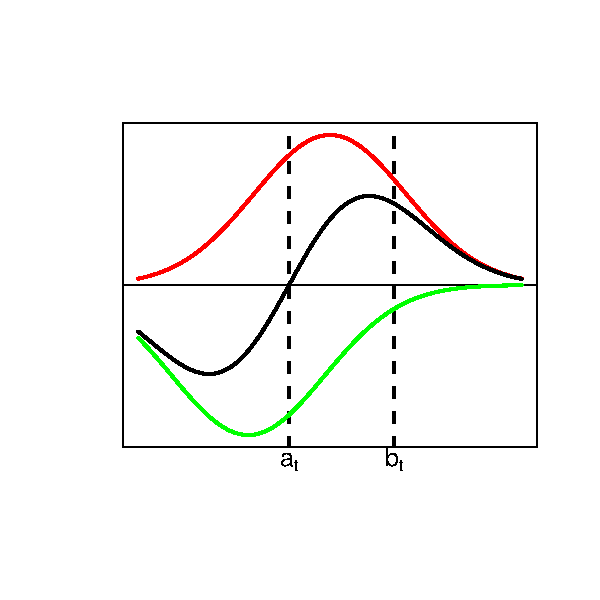
\includegraphics[scale=0.75]{g1.pdf}
%	\caption{The fundamental solution centered on $y_{t-1}$ plus a negated fundamental solution reflected about $a_t$. Here, $\sigma = 3$, $a_t = -1$ and $b_t = 1$.}
%	\label{fig:g1}
%\end{figure}

If we reflect $g_1$ about $b_t$ via a translation of the mean $\xi(y) = 2b_t - y$ and a negation:

\[ r_1(y,s) = -N(y; \xi(y_t), s\sigma^2) + N(y; \xi(\zeta(y_t)), s\sigma^2) \]

 and add this reflection to $g_1$

\[ g_2(y,s) = g_1(y,s) + r_1(y,s) = N(y; y_t, s\sigma^2) - N(y; \zeta(y_t), s\sigma^2) -N(y; \xi(y_t), s\sigma^2) + N(y; \xi(\zeta(y_t)), s\sigma^2), \] 
the resultant function $g_2$ (Figure (\ref{fig:g2})) also satisfies the heat equation and it matches the boundary condition at $b_t$, but the boundary condition at $a_t$ no longer holds. The process can be continued in this manner iteratively, with each reflection enforcing the boundary condition at $a_t$ then $b_t$. However, it is necessary to ensure that the reflections do not contain images already in the system of images.

Each reflection sends the sources of the reflected fundamental solutions further away from the domain $[a_t, b_t]$, making the maximal factor by which the boundary conditions are violated less and less. Thus, we can write down the solution to the IC/BV problem as the infinite sum of the superposition of reflected fundamental solutions. This can be defined by all possible alternating combinations of $\xi$ and $\zeta$ applied to the center of $g_0$. The expression in (\ref{eq:images}) enumerates all such combinations and is therefore the solution to the diffusion equation under the initial conditions and boundary values. 
%
\begin{align}
	p(y,s) &= N( y ; y_{t-1}, s\sigma^2) - N( y ; \zeta(y_{t-1}), s\sigma^2) - N( y ; \xi(y_{t-1}), s\sigma^2) + \nonumber \\
		& \quad \sum_{n=1}^\infty \left[ N( y ; (\xi \circ \zeta)^n (y_{t-1}), s\sigma^2) + N(y ; (\zeta \circ \xi)^n (y_{t-1}), s\sigma^2 ) \right. \nonumber \\
		&  \qquad \qquad \left. -  N( y ; (\xi \circ \zeta)^n \circ \xi (y_{t-1}), s\sigma^2) - N( y ; (\zeta \circ \xi)^n \circ \zeta (y_{t-1}), s\sigma^2) \right]. \label{eq:images}
\end{align}
%
The final solution to the original advection-diffusion problem is therefore $p(y,s)$ multiplied by the exponential factor $\exp(ay+bs)$, which is given in equation(\ref{eq:q-final-images}). Figure (\ref{fig:g3}) shows the solution from equation (\ref{eq:images}) with $n=1$. 

%\begin{figure}
%	\centering
%	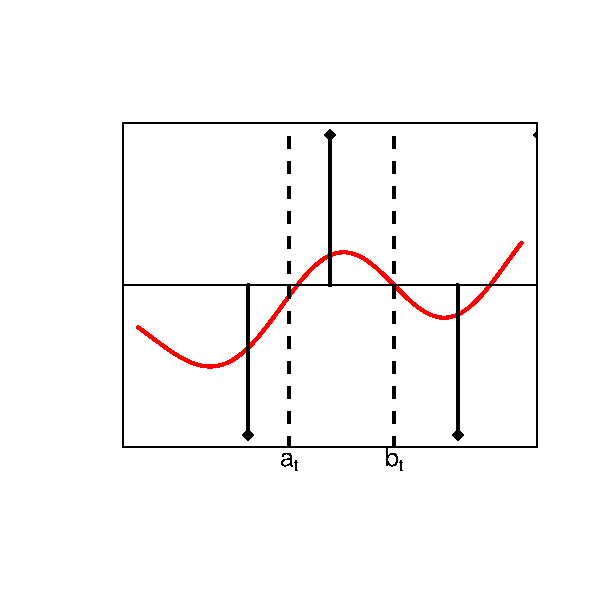
\includegraphics[scale=0.75]{g2.pdf}
%	\caption{The solution obtained by a reflection about $a_t$ then $b_t$.}
%	\label{fig:g2}
%\end{figure}

%\begin{figure}
%	\centering
%	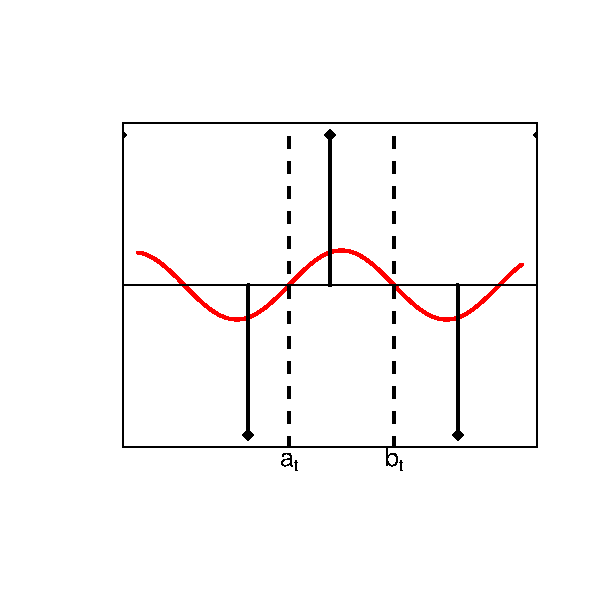
\includegraphics[scale=0.75]{g3.pdf}
%	\caption{The solution obtained by a reflection about $a_t$ then $b_t$.}
%	\label{fig:g3}
%\end{figure}

\begin{figure}[htbp]
        \centering
        \begin{subfigure}[t]{0.3\textwidth}
                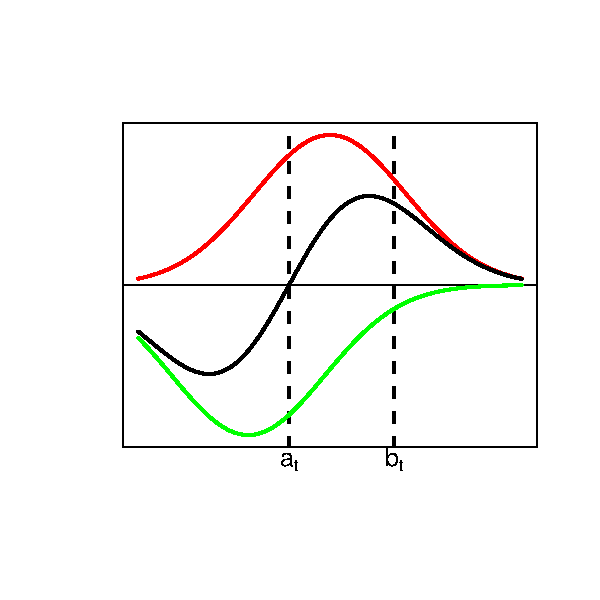
\includegraphics[width=\textwidth]{g1.pdf}
                \caption{The fundamental solution $g_0$ (red), its reflection about $a_t,$ $r_0$ (green), and their sum $g_1$ (black). Observe that the boundary condition is satisfied at $a_t$ but not $b_t$.}
                \label{fig:g1}
        \end{subfigure}%
        ~ %add desired spacing between images, e. g. ~, \quad, \qquad, \hfill etc.
          %(or a blank line to force the subfigure onto a new line)
        \begin{subfigure}[t]{0.3\textwidth}
                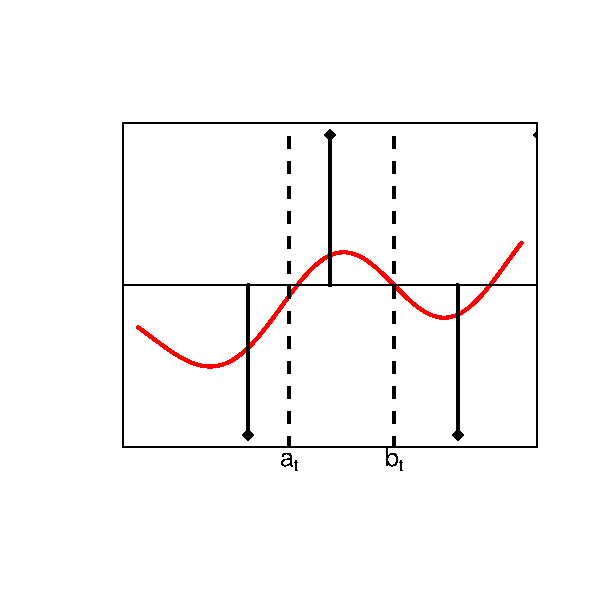
\includegraphics[width=\textwidth]{g2.pdf}
                \caption{The solution after a single reflection about $a_t$, $g_1$ (red), its reflection about $b_t$, $r_1$ (green), and their sum $g_2$ (black). The boundary condition is satisfied at $b_t$ but is now violated at $a_t$.}
                \label{fig:g2}
        \end{subfigure}
        ~ %add desired spacing between images, e. g. ~, \quad, \qquad, \hfill etc.
          %(or a blank line to force the subfigure onto a new line)
        \begin{subfigure}[t]{0.3\textwidth}
                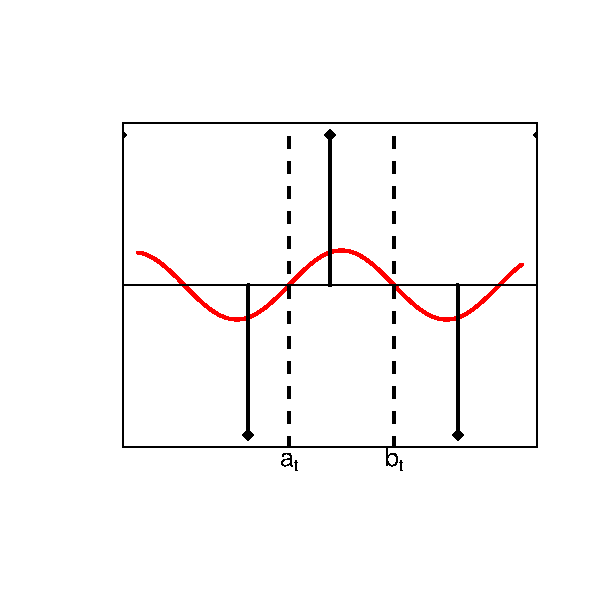
\includegraphics[width=\textwidth]{g3.pdf}
                \caption{The solution according to equation (\ref{eq:images}) with $n=1$. }
                \label{fig:g3}
        \end{subfigure}
        \caption{Construction of the solution using the Method of Images}\label{fig:animals}
\end{figure}

\begin{eqnarray}
	q(y,s) &=& \exp\left( \frac{\sqrt{2\mu}}{\sigma} y \right) \times \nonumber \\
		&& \Bigg\{ N( y ; y_{t-1}, s\sigma^2) - N( y ; \zeta(y_{t-1}), s\sigma^2) - N( y ; \xi(y_{t-1}), s\sigma^2) + \nonumber \\
		&& \quad \sum_{n=1}^\infty \left[ N( y ; (\xi \circ \zeta)^n (y_{t-1}), s\sigma^2) + N(y ; (\zeta \circ \xi)^n (y_{t-1}), s\sigma^2 ) \right. \nonumber \\
		& & \qquad \left. -  N( y ; (\xi \circ \zeta)^n \circ \xi (y_{t-1}), s\sigma^2) - N( y ; (\zeta \circ \xi)^n \circ \zeta (y_{t-1}), s\sigma^2) \right] \Bigg\} . \label{eq:q-final-images} 
\end{eqnarray}

%the above partial differential equation becomes
%\[ \Phi'(s)f(y) = \frac{1}{2}\sigma^2 \Phi(s) f''(y) \]
%Isolating functions of $s$ and $y$, we see that the ratios of the solution functions and their respective derivatives must be equal to a constant independet of the two variables
%\[ \frac{\Phi'(s)}{\Phi(s)} = \frac{1}{2}\sigma^2 \frac{f''(y)}{f(y)} = \frac{1}{\lambda}. \]
%The solution to the time-dependent problem is $\Phi(s) = \Phi(0)\exp(\lambda t)$. For the solution to be defined over all $t$, we need $\lambda < 0$. The spatial problem, a second-order linear differential equation 
%\[ f''(y) = \frac{2}{\sigma^2 \lambda} f(y) = -\frac{2}{\sigma^2 |\lambda|} f(y) \]
%is satisfied by the linear combination
%\[ f(y) = A\sin\left( y\sqrt{\frac{2}{\sigma^2 |\lambda| }} \right) + B\cos\left( y\sqrt{\frac{2}{\sigma^2 |\lambda| }} \right), \]
%where we require at least one of $A$ and $B$ be nonzero. In addition to satisfying the differential equation, $f(y)$ must also satisfy the boundary contions. Hence,
%\begin{eqnarray*}
%	f(a_t) &=&  A\sin\left( a_t\sqrt{\frac{2}{\sigma^2 |\lambda|}} \right) + B\cos\left( a_t\sqrt{\frac{2}{\sigma^2 |\lambda|}} \right) = 0, \\
%	f(b_t) &=&  A\sin\left( b_t\sqrt{\frac{2}{\sigma^2 |\lambda|}} \right) + B\cos\left( b_t\sqrt{\frac{2}{\sigma^2 |\lambda|}} \right) = 0. 
%\end{eqnarray*}
%
%We can re-scale the problem by a shift of $a_t$ so that $a_t \to 0$ and $b_t \to b_t - a_t \equiv L$. Let $\xi \equiv y - a_t$. Under this transformation, we have 
%\begin{eqnarray*}
%	B &=& 0, \\
%	A\sin\left( L\sqrt{\frac{2}{\sigma^2 |\lambda|}} \right) + B\cos\left( L\sqrt{\frac{2}{\sigma^2 |\lambda|}} \right) &=& 0. 
%\end{eqnarray*}
%Therefore, $B=0$, which forces $A \neq 0$. It follows that $\sin\left( L\sqrt{\frac{2}{\sigma^2 |\lambda|}} \right) = 0$, which means that
%\[ L\sqrt{\frac{2}{\sigma^2 |\lambda|}}  = n\pi, \quad n=1, \ldots \quad ( n \neq 0 \mbox{ because } L \neq 0 ) \]
%Since $n$ goes over the integers, there is a countable number of constants, or \textit{modes}, $\lambda_n$ for our problem, given by
%\[ \lambda_n = -\frac{2L^2}{n^2 \pi^2 \sigma^2 }. \]
%Thus, the solution to the problem, both in time and space, is given by the sum of basis functions for each mode
%\[ p(\xi, t) = \sum_{n=1}^\infty \Phi_n(t) f_n(\xi ) = \sum_{n=1}^\infty \Phi_n(0) \exp\left( -\frac{2L^2}{n^2 \pi^2 \sigma^2 } t \right) A_n \sin\left( \xi \sqrt{\frac{2}{\sigma^2 \frac{2L^2}{n^2 \pi^2 \sigma^2 }}} \right) = \sum_{n=1}^\infty \tilde{A}_n \exp\left( -\frac{2L^2}{n^2 \pi^2 \sigma^2 } t \right) \sin\left( \xi \frac{n\pi}{L} \right). \]
%Expressing the solution in terms of $y$ instead of $\xi$,
%\[ p(y,t) =  \sum_{n=1}^\infty \tilde{A}_n \exp\left( -\frac{2L^2}{n^2 \pi^2 \sigma^2 } t \right) \sin\left( (y-a_t) \frac{n\pi}{L} \right). \]

%There are a few things that must be observed of this solution. First, the constants $\Phi_n(0)$ and $A_n$ have been combined into $\tilde{A}_n$, which is determined by the sine series representation for the initial condition, $\delta(y - y_t)$. This will be dealt with below. Second, the contribution of each additional mode decays at the order of $\exp(-1/n^2)$, making the approximation of $p(y,t)$ in terms of a finite number of terms very efficient. Finally, the solution behaves as expected: $p(y,t) \to 0$ as $t \to \infty$. This corresponds to the intuition that as time progresses a particle is less likely to stay bounded between the values $a_t$ and $b_t$. 


\section{Finding the Likelihood for the Closing Price}
The full solution $q(y,t)$ is the likelihood that a random process satisfying the stochastic differential equation (\ref{eq:SDE}) has an infimum greater than or equal to $a_t$ and a supremum less than or equal to $M_t$ over the period $(t-1, t)$.  In terms of probabilities
\[
	q(y,t) = P( m_t \geq a_t, M_t \leq b_t, Y_t = y | Y_{t-1} = y_{t-1}, m_t < M_t ).
\]
%
However, to perform the statistical inference we need the density associated with $q(y,t)$, which is derived by differentiating $q(y,t)$ with respect to the boundary conditions:
\begin{equation} -\frac{\partial^2 }{\partial a_t \partial b_t } q(y,t) = P( m_t = a_t, M_t = b_t, Y_t = y | Y_{t-1} = y_{t-1}). \label{eq:likelihood}
\end{equation}
%
The analytic expression for the likelihood, whether that in equation (\ref{eq:q-final}) or (\ref{eq:q-final-images}), allows us to perform this differentiation numerically as well as analytically. Once this differentiation is performed, we can use familiar optimization methods to find maximum likelihood estimates for the parameters $\mu$ and $\sigma^2$, given closing, open, high, and low prices for a given interval $(t-1,t)$. 

\subsection{Evaluating the accuracy of the solutions}

We want to compare the convergence of the likelihood (\ref{eq:likelihood}) based on the trigonometric expansion solution (\ref{eq:q-final}). This convergence is dependent upon the number of terms used in the truncated summation for the expansion, as well as the size of the discrete step when performing numerical differentiation. This analysis sets the stage for our treatment of the bivariate advection-diffusion problem in Chapter 3.

Considered are ten simulations over a nominal period of length 1 based on a forward-Euler discretization scheme of the governing stochastic differential equation:
\begin{equation} 
	Y_{k+1} = Y_{k} + \mu \Delta t^* + \sigma \Delta t^* \epsilon_k, \label{eq:SDE-discrete}
\end{equation}
with $\Delta t^* = 1/23,400$,  and $\epsilon_k \sim N(0,1)$. This is equivalent to sampling the returns once every second over the length of a trading day. Further, 
\[ \mu = 1, \qquad \sigma = 1. \]
For each simulation there is a recorded min, max, and closing value, while all log open prices are set to 0. As a test to study the numerical accuracy of the solution, we examine the likelihood value at the closing log return using the observed minima and maxima set to $a_t$ and $b_t$ respectively, as well as the true $\mu$ and $\sigma$ used to generate the data. When performing numerical differentiation, a second-order two-point stencil method is used with a discretization step
\[ 
	\Delta x = \frac{1}{2^k} \frac{1}{100} (b_t - a_t).
\]
Values of the likelihoods are considered across ranges of $N$ and $k$ and are compared to the likelihood values obtained through analytic differentiation. The results are shown in Tables (\ref{table:m4}) - (\ref{table:analytic}). We see that for both numerical differentiation factors $k=4$ and $k=8$ likelihood values match with those obtained via analytic differentiation, so either differentiation approach is appropriate for maximum likelihood estimation. Further, we see that likelihood values are the same across all sizes of $N$. This means that the number of terms needed in the trigonometric expansion for accurate solutions is relatively low, and the Fourier expansion used in our derivation is an efficient representation for the univariate diffusion problem.

\begin{table}
	\centering
	\csvautotabular{./chapter-2-univariate-case/table-m-4.csv}
	\caption{Likelihood values for simulations obtained via numerical differentiation with $k=4$ ($\Delta x = 1/(100 \cdot 2^4) \cdot (b_t-a_t)$). }
	\label{table:m4}
\end{table}

\begin{table}
	\centering
	\csvautotabular{./chapter-2-univariate-case/table-m-8.csv}
	\caption{Likelihood values for simulations obtained via numerical differentiation with $k=8$ ( $\Delta x = 1/(100 \cdot 2^8) \cdot (b_t-a_t)$). }
	\label{table:m8}
\end{table}

\begin{table}
	\centering
	\csvautotabular{./chapter-2-univariate-case/table-analytic.csv}
	\caption{Likelihood values for simulations obtained via analytic differentiation. }
	\label{table:analytic}
\end{table}


\section{Using Close, High, Low, Open Data for High-Frequency Data: a Monte Carlo Simulation Study}
For high-frequency data where transactions occur on the microsecond scale, there is a lot of available information even within sampling intervals on the second scale. Realized volatility estimates use all data within sampling intervals, while the estimates based on the likelihood developed above use summaries of intraperiod data in the form of open, close, high, and low (OCHL) recorded prices. In this simulation study, we are interested in seeing how our maximum likelihood estimates for $\sigma^2$ based on OCHL data compare with RV estimates.

%Discussed previously was the Realized Volatility estimator, which is a model-free estimator for the integrated volatility of a process over an interval $\Delta$. In the absence of microstructure noise, we know that $RV \to \int_{t-1}^t \sigma^2(y_s,s)dW = \sigma^2$ (for a constant $\sigma^2$ over $\Delta = (t-1,t)$) as the number of samples over the interval $(t-1,t)$ goes to infinity. Precisely because of this limiting property, the RV estimator is widely used in the estimation of volatility models with high-frequency data. In addition to the standard RV estimator in equation (\ref{eq:RV}), we will consider an RV estimator which attempts to overcome the bias introduced by microsctructure noise. 
%
%We are interested in seeing how our maximum likelihood estimates for $\sigma^2$ based on open, close, high, and low (OCHL) data compare with RV estimates. We consider two simulation-based scenarios, one with and one without microstructure noise. 
%
\subsection{Maximum Likelihood Estimation}
The goal of the simulation study is to understand the trade-offs between using all high-frequency data and, instead, using summaries. Recalling the basic diffusion model in (\ref{eq:SDE}) with constant $\mu$ and $\sigma^2$, the simulations use 
\[ \mu = 7.936508 \cdot 10^{-5}, \qquad \sigma = 0.01259882. \]
The parameters correspond to daily estimates for drift and standard deviation of the returns of the S\&P 500 index. Thus, in our simulations $\Delta$ corresponds to an idealized 7-hour trading day. The simulated data is obtained by the forward-Euler discretization in equation (\ref{eq:SDE-discrete}), where $\epsilon_k \sim N(0,1)$, and index $k$ corresponds to the time $k \Delta t^* $, and $\Delta t^*$ corresponds to a second of a trading day. Generating the data according to equation (\ref{eq:SDE-discrete}) amounts to sampling the diffusion process every second. It should be noted here that the data-generation method used here does not include microstructure noise.

When performing estimation, longer sampling intervals are used. They are  
\[ \Delta t = 5 \mbox{ sec}, 10 \mbox{ sec}, 20 \mbox{ sec}, 30 \mbox{ sec}, 1 \mbox{ min}, 5  \mbox{ min}, 10 \mbox{ min}, 20 \mbox{ min}, 30 \mbox{ min}, 1 \mbox{hr}, 3.5 \mbox{hr}, 7 \mbox{hr}. \]
We expect the realized volatility estimate to approach the true diffusion parameter, in probability, as $\Delta t \to 0$. As for estimating volatility using OCHL data, each simulated day contains $1/\Delta t$ intervals. Each interval $[k\Delta t, (k+1)\Delta t]$, in turn, contains $\Delta t/\Delta t^* + 1$ data points. For example, if $\Delta t = 5\mbox{ sec}$, there are six data points in the interval $[k\Delta t, (k+1)\Delta t]$: the price observed at time $k \Delta t$, and a price every second up to, and including, time $(k+1) \Delta t$. The price at time $k\Delta t$ is the opening price, the price at time $(k+1)\Delta t$ is the closing price, and the minimum and maximum prices observed in the samples between are used as $a_t$ and $b_t$ respectively for the likelihood in (\ref{eq:likelihood}). Using this data and the analytic expression for the likelihood, we optimize over $\mu$ and $\sigma^2$ to find the maximum likelihood estimates for the parameters. Thus, for every simulated day for a given $\Delta t$, there is an independent set of estimates for $\sigma^2$ and $\mu$. 

The results for 1000 simulated trading days are shown in Figure (\ref{fig:estimator-comparison-no-microstructure}). We see that, for the shortest sampling periods, the realized volatility estimator outperforms the OCHL estimator in terms of both bias and mean-squared error, as expected. However, the variance of the RV estimator is much greater than that of the OCHL estimator. As a result, the OCHL estimator quickly overtakes the RV estimator in terms of MSE performance.

It is notable that the OCHL estimator has a large bias for small sampling periods. As long as the observations of a diffusion process are finite in number, the observed maximum is less than or equal to the true maximum and the observed minimum is greater than or equal to the true minimum. The discrepancy between the true and observed extreme values becomes greater as the number of observations becomes smaller. This artificially smaller range between extreme values biases the estimates for volatility to be below the true value for smaller intervals $[k\Delta t, (k+1)\Delta t]$ since they contain fewer data points. 

\begin{figure}
	\centering
	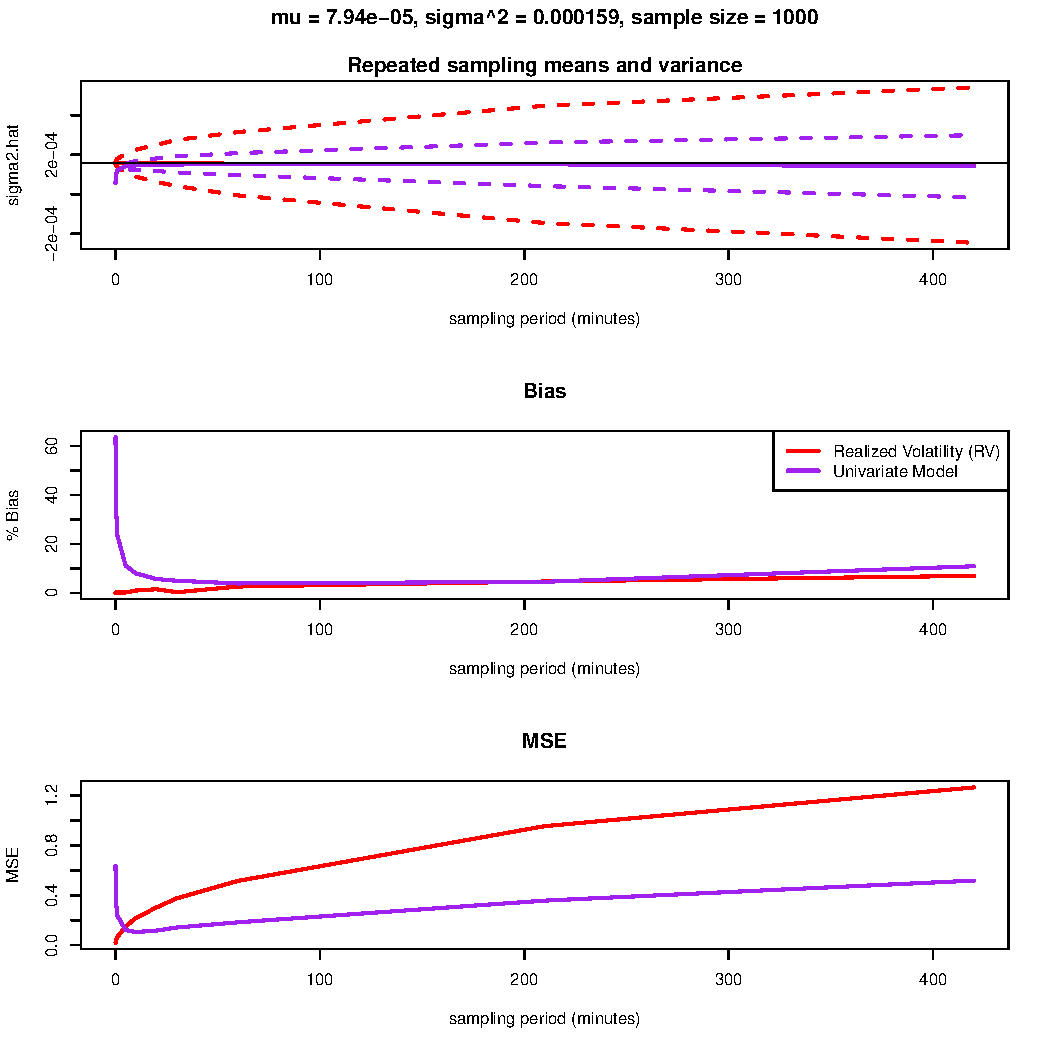
\includegraphics[scale=0.8]{results-7-14-13-5-53.pdf}
	\caption{Results for 1000 trading days}
	\label{fig:estimator-comparison-no-microstructure}
\end{figure}

%\subsection{Estimation With Microstructure Noise}
%It is important to examine how robust the RV and OCHLO estimators are to microstructure noise. The confounding phenomenon is introduced through the data generating process as an additional noise term: 
%\begin{equation} 
%	Y_{k+1} = Y_{k} + \mu \Delta t^* + \sigma \Delta t^* \epsilon_k + \gamma \nu_k, \label{eq:SDE-discrete-noise}
%\end{equation}
%with $\nu_k \sim N(0,1)$. Considered are a number of magnitudes for the noise term $\gamma$. It should be noted that the noise added to the observation does not scale with observation periods. This means that for short intervals, $\gamma$ can dominate the diffusion process, but as the sampling interval $\Delta t$ increases, $\gamma$ becomes negligible with respect to the diffusion variance $(\sigma \Delta t)^2$. This is precisely the empirical market dynamics of microstructure noise. Thus, we expect both types of estimators to perform as above for bigger $\Delta t$, but of particular interest are shorter sampling intervals. 

\chapter{Range-Based Methods for High-Frequency Data In Two Dimensions} \label{chapter:3}

\section{Motivation}
Just as using the range of an asset, as opposed to only opening and closing values, improves the estimation of drift and volatility, we expect that using OCHL data for two assets can improve estimates for drift and volatility, as well as the estimate of their correlation. Accurate estimation of correlation across assets plays a key role in portfolio theory, as it allows for portfolio diversification to reduce risk. 

\section{Problem Formulation}
In the two-dimensional case, we simply extend the geometric Brownian motion model used in Chapter 2 to two dimensions:

\begin{eqnarray}
	dY_{1,s} = \mu_1 ds + \sigma_1 dW_{1,s}, \\ \label{eq:SDE-1}
	dY_{2,s} = \mu_2 ds + \sigma_2 dW_{2,s}. \label{eq:SDE-2}
\end{eqnarray}
Here we introduce correlation $\rho$ in the log prices of the two assets:
\[ Cov(W_1, W_2) = \rho. \]

Again using the Fokker-Planck Equation, we can take the system of SDEs in (\ref{eq:SDE-1}) - (\ref{eq:SDE-2}) and express the probability density of the asset price $q(y_1, y_2,s)$ as the PDE
\begin{eqnarray}
	\frac{\partial}{\partial s} q(y,s) &=& -\mu_1 \frac{\partial}{\partial y_1}q(y_1, y_2,s) -\mu_1 \frac{\partial}{\partial y_2}q(y_1, y_2,s) \nonumber \\
		&&  + \frac{1}{2}\sigma_1^2 \frac{\partial^2}{\partial y_1^2} q(y_1, y_2,s) + \frac{1}{2} \sigma_2^2 \frac{\partial^2}{\partial^2 y_2}q(y_1,y_2,s) + \rho \sigma_1 \sigma_2 \frac{\partial^2}{\partial y_1 \partial y_2} q(y_1, y_2, s) \label{eq:ch3-IV-1} \\
	q(y_1, y_2, t-1) &=& \delta(y_1-y_{1,t-1})\delta(y_2-y_{2,t-1}), \label{eq:ch3-IV-2}
\end{eqnarray}
where $y_{1,t-1}$ and $y_{2,t-1}$ are the prices at the beginning of the interval, and $\delta$ is the Dirac delta function. As in Chapter 2, we introduce the maximum and minimum observed prices of each asset, which establish the boundary conditions for the two-dimensional IC/BV problem

\begin{eqnarray}
	\frac{\partial}{\partial s} q(y,s) &=& -\mu_1 \frac{\partial}{\partial y_1}q(y_1, y_2,s) -\mu_1 \frac{\partial}{\partial y_2}q(y_1, y_2,s) \nonumber \\
		&&  + \frac{1}{2}\sigma_1^2 \frac{\partial^2}{\partial y_1^2} q(y_1, y_2,s) + \frac{1}{2} \sigma_2^2 \frac{\partial^2}{\partial^2 y_2}q(y_1,y_2,s) + \rho \sigma_1 \sigma_2 \frac{\partial^2}{\partial y_1 \partial y_2} q(y_1, y_2, s) \label{eq:ch3-IC-BV-1} \\
	q(y_1, y_2, t-1) &=& \delta(y_1-y_{1,t-1})\delta(y_2-y_{2,t-1}), \label{eq:ch3-IC-BV-2} \\
	q(y_1, y_2, s) &=& 0 \quad \mbox{for} \quad y_1 = a_{1,t}, b_{1,t} \,\, \mbox{ or } \,\, y_2 = a_{2,t}, b_{2,t}. \label{eq:ch3-IC-BV-3}
\end{eqnarray}

We use the same treatment as in Chapter 2 to transform the advection-diffusion problem in equations (\ref{eq:ch3-IC-BV-1}) - (\ref{eq:ch3-IC-BV-3}) into a purely diffusion problem. Letting $\mathbf{a} = (a_1, a_2)^T$ and $\mathbf{y} = (y_1, y_2)^T$, we once again introduce the form 
%
\[ q(\mathbf{y}, s) = \exp(\mathbf{a}^T\mathbf{y} + bs)p(\mathbf{y}, s). \]
%
Substituting the expression into the left and right-hand sides of (\ref{eq:ch3-IC-BV-1}) and equating gives us an expression for $\mathbf{a}$ and $b$ which eliminate the zeroeth and first order derivatives of $p$:

\[ b = \mu_1 a_1 + \mu_2 a_2 - \frac{1}{2}\sigma^2_1 a_1^2 - \frac{1}{2}\sigma^2_2 a_2^2 + \rho\sigma_1 \sigma_2 a_1 a_2, \]

\[ \left( \begin{array}{cc}
		\sigma_1^2 & \rho\sigma_1 \sigma_2 \\
		\rho\sigma_1 \sigma_2 & \sigma^2_2 
 \end{array} \right) \left( \begin{array}{c}
					a_1 \\ a_2 \end{array} \right) = \left( \begin{array}{c} \mu_1 \\ \mu_2 \end{array} \right). \]
Under these conditions, the advection-diffusion problem is once again reduced to a pure diffusion problem on a bounded domain:
\begin{eqnarray}
	\frac{\partial p(\mathbf{y},s)}{\partial s} &=& \frac{1}{2}\sigma_1^2 \frac{\partial^2}{\partial y_1^2} p(\mathbf{y},s) + \frac{1}{2} \sigma_2^2 \frac{\partial^2}{\partial^2 y_2}p(\mathbf{y},s) + \rho \sigma_1 \sigma_2 \frac{\partial^2}{\partial y_1 \partial y_2} p(\mathbf{y}, s), \label{eq:ch3-heat-1} \\
	p(\mathbf{y}, t-1) &=& \delta(y_1-y_{1,t-1})\delta(y_2-y_{2,t-1}), \label{eq:ch3-heat-2} \\
	p(\mathbf{y}, s) &=& 0 \quad \mbox{for} \quad y_1 = a_{1,t}, b_{1,t} \,\, \mbox{ or } \,\, y_2 = a_{2,t}, b_{2,t}. \label{eq:ch3-heat-3}
\end{eqnarray}


\section{Solution with the Method of Images}
Our first attempt to solve the two-dimensional diffusion problem was to apply the Method of Images approach in Chapter 2. The fundamental solution to the diffusion problem on an unbounded domain is the bivariate normal density with mean and covariance matrix 
\[ \boldsymbol{\mu} = (y_{1,t-1}, y_{2,t-1})^T, \qquad \boldsymbol{\Sigma} = \left( \begin{array}{cc}
															\sigma_1^2 & \rho \sigma_1 \sigma_2 \\
															\rho \sigma_1 \sigma_2 & \sigma_2^2 		
															\end{array} \right). \]
However, reflection of the fundamental solution across a certain boundary produces an image which satisfies a diffusion equation with a \textit{negated} correlation coefficient $\rho$ (Figure (\ref{fig:unmodified-reflection})), so that the differential equation satisfied by the reflected function is no longer the original PDE (note the minus sign in front of the mixed derivative term): 
\[ 
	\frac{\partial p(\mathbf{z},s)}{\partial s} = \frac{1}{2}\sigma_1^2 \frac{\partial^2}{\partial z_1^2} p(\mathbf{z},s) + \frac{1}{2} \sigma_2^2 \frac{\partial^2}{\partial^2 z_2}p(\mathbf{z},s) - \rho \sigma_1 \sigma_2 \frac{\partial^2}{\partial z_1 \partial z_2} p(\mathbf{z}, s)
\]
Hence, the summation of reflected images, although satisfying the boundary conditions in the limiting case, does not satisfy the original PDE. 

One can eliminate the correlation term $\rho$ through a change of coordinates consisting of a rotation, given by the eigenvalue decomposition of the covariance matrix, and a translation, such that the diffusion problem is reduced even further to
\[
\frac{\partial p(\boldsymbol{\zeta},s)}{\partial s} = \frac{1}{2}\tilde{\sigma}_1^2 \frac{\partial^2}{\partial \zeta_1^2} p(\boldsymbol{\zeta},s) + \frac{1}{2} \tilde{\sigma}_2^2 \frac{\partial^2}{\partial^2 \zeta_2}p(\boldsymbol{\zeta},s).
\]
However, the boundary where the solution is zero is no longer a rectangle but is instead a parallelogram. The non-orthogonality of the boundaries makes the process of reflecting the fundamental solution about the boundaries problematic. Particularly, if the angles between intersecting sides are not factors of $\pi$, repeated reflection places images within the computational domain of the problem, thereby violating the initial condition (see Figure (\ref{fig:transformed-reflection})). 

\begin{figure}[htbp]
        \centering
        \begin{subfigure}[t]{0.4\textwidth}
                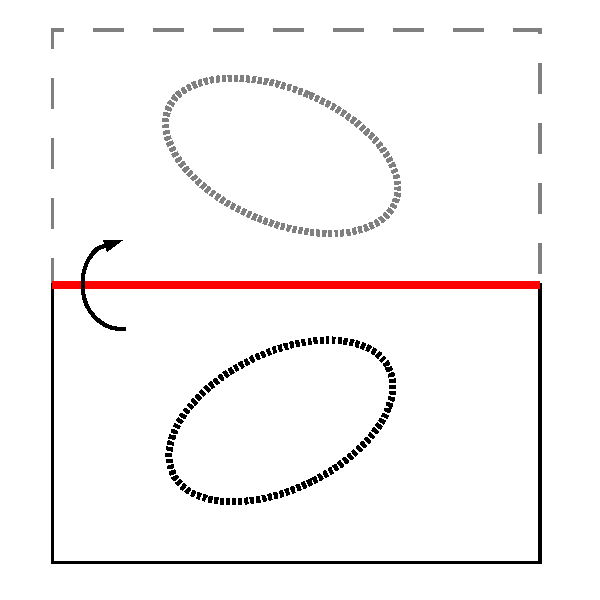
\includegraphics[width=\textwidth]{./chapter-3-two-dimensional-case/unmodified-reflection.pdf}
                \caption{When the fundamental solution (covariance ellipsoid in black) is reflected across the red boundary, the reflection has a covariance ellipsoid (gray) with a negative slope, meaning that the reflection satisfies a PDE where the correlation coefficient is negative. The sum of the fundamental solution and the reflection satisfies the boundary condition over the red line but does not satisfy the governing PDE.}
                \label{fig:unmodified-reflection}
        \end{subfigure}%
        \quad %add desired spacing between images, e. g. ~, \quad, \qquad, \hfill etc.
          %(or a blank line to force the subfigure onto a new line)
        \begin{subfigure}[t]{0.4\textwidth}
                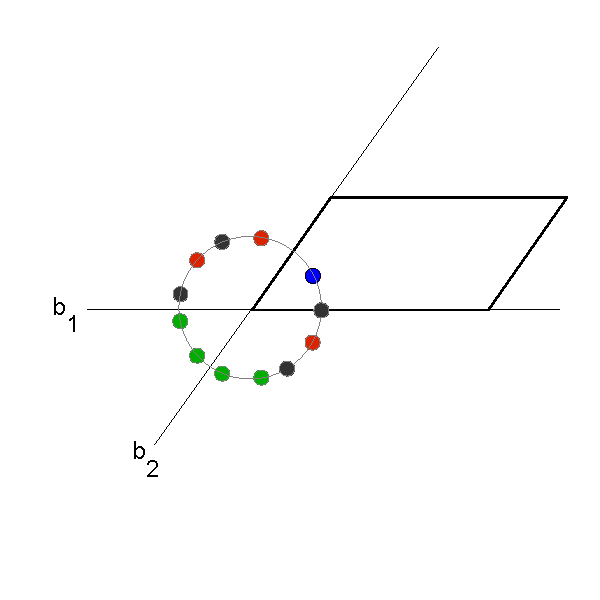
\includegraphics[width=\textwidth]{./chapter-3-two-dimensional-case/transformed-reflection.pdf}
                \caption{The fundamental solution, centered on the initial condition and denoted by the blue-inscribed red disk, is reflected alternatively around the boundaries $b_1$ and $b_2$. The displayed system of images is the results of three successive pairs of reflections around $b_1$ then $b_2$, with red corresponding to the first, green to the second, and black to the third set of reflections. We see that the system includes a fundamental solution in the computational domain in additional to the original, thereby violating the initial conditions of the problem. }
                \label{fig:transformed-reflection}
        \end{subfigure}
        
        \caption{Construction of the solution using the Method of Images}\label{fig:animals}
\end{figure}

\section{Solution by Fourier Expansion}
Similarly to the approach in Chapter 2, equation (\ref{eq:trig-expansion}), we offer a solution to the diffusion problem in terms of a trigonometric expansion of sine functions, since the basis functions must satisfy the boundary conditions:
\begin{equation}
	p(\mathbf{y}, s) = \sum_{m=1}^\infty \sum_{n=1}^\infty C_{m,n}(s) \sin\left( \frac{m \pi (y_1 - a_{1,t})}{b_{1,t} - a_{1,t}} \right) \sin\left( \frac{n \pi (y_2 - a_{2,t})}{b_{2,t} - a_{2,t}} \right)
\end{equation}	

We substitute the above form into equation (\ref{eq:ch3-heat-1}) in order to obtain expressions for $C_{m,n}(t)$:
\begin{eqnarray}
	\lefteqn{ \sum_{m=1}^\infty \sum_{n=1}^\infty \frac{dC_{m,n}(s)}{ds} \sin\left( \frac{m \pi (y_1 - a_{1,t})}{b_{1,t} - a_{1,t}} \right) \sin\left( \frac{n \pi (y_2 - a_{2,t})}{b_{2,t} - a_{2,t}} \right) =   } \nonumber \\
	&& \frac{1}{2}\sigma^2_1 \sum_{m=1}^\infty \sum_{n=1}^\infty C_{m,n}(s) \left( \frac{m\pi}{b_{1,t}-a_{1,t}} \right)^2 \sin\left( \frac{m \pi (y_1 - a_{1,t})}{b_{1,t} - a_{1,t}} \right) \sin\left( \frac{n \pi (y_2 - a_{2,t})}{b_{2,t} - a_{2,t}} \right) \nonumber \\
	&+&  \frac{1}{2}\sigma^2_2 \sum_{m=1}^\infty \sum_{n=1}^\infty C_{m,n}(s) \left( \frac{n\pi}{b_{2,t}-a_{2,t}} \right)^2 \sin\left( \frac{n \pi (y_1 - a_{1,t})}{b_{1,t} - a_{1,t}} \right) \sin\left( \frac{n \pi (y_2 - a_{2,t})}{b_{2,t} - a_{2,t}} \right) \nonumber \\
	&+& \rho \sigma_1 \sigma_2 \sum_{m=1}^\infty \sum_{n=1}^\infty C_{m,n}(s) \left( \frac{m\pi}{b_{1,t}-a_{1,t}} \right) \left( \frac{n\pi}{b_{2,t}-a_{2,t}} \right) \cos\left( \frac{m \pi (y_1 - a_{1,t})}{b_{1,t} - a_{1,t}} \right) \cos\left( \frac{n \pi (y_2 - a_{2,t})}{b_{2,t} - a_{2,t}} \right) \label{eq:expanded}
\end{eqnarray}

To deal with the cosine terms, we expand them in terms of sine functions as well, obtaining

\[
	\cos\left( \frac{m \pi (y_1 - a_{1,t})}{b_{1,t} - a_{1,t}} \right) \cos\left( \frac{n \pi (y_2 - a_{2,t})}{b_{2,t} - a_{2,t}} \right) = \sum_{k = 1}^\infty \sum_{j=1}^\infty d_{k}^{(m)} d_{j}^{(n)} \sin\left( \frac{k \pi (y_1 - a_{1,t})}{b_{1,t} - a_{1,t}} \right)\sin\left( \frac{j \pi (y_2 - a_{2,t})}{b_{2,t} - a_{2,t}} \right).
\]

Using the orthogonality of the sine and cosine series with respect to the $L^1$ norm

\[
	d^{(m)}_k = \left\{ \begin{array}{cr} 0 & \mbox{ if } k-m = \mbox{ even} \\
			\frac{4k}{\pi(k^2 - m^2)} & \mbox{ if } k-m = \mbox{ odd.} \end{array} \right.
\]
Focusing on the last line with the cosine terms
\begin{eqnarray}
	\lefteqn{ \rho \sigma_1 \sigma_2 \sum_{m=1}^\infty \sum_{n=1}^\infty C_{m,n}(s) \left( \frac{m\pi}{b_{1,t}-a_{1,t}} \right) \left( \frac{n\pi}{b_{2,t}-a_{2,t}} \right) \cos\left( \frac{m \pi (y_1 - a_{1,t})}{b_{1,t} - a_{1,t}} \right) \cos\left( \frac{n \pi (y_2 - a_{2,t})}{b_{2,t} - a_{2,t}} \right) } \label{eq:ch3-mixed-term} \\
%	&=& \rho \sigma_1 \sigma_2 \sum_{m=1}^\infty \sum_{n=1}^\infty C_{m,n}(t) \left( \frac{m\pi}{b_{1,t}-a_{1,t}} \right) \left( \frac{n\pi}{b_{2,t}-a_{2,t}} \right) \sum_{k = 1}^\infty \sum_{j=1}^\infty d_{k}^{(m)} d_{j}^{(n)} \sin\left( \frac{k \pi (y_1 - a_{1,t})}{b_{1,t} - a_{1,t}} \right)\sin\left( \frac{j \pi (y_2 - a_{2,t})}{b_{2,t} - a_{2,t}} \right) \nonumber \\
	&=& \rho \sigma_1 \sigma_2 \sum_{m=1}^\infty \sum_{n=1}^\infty \sum_{k = 1}^\infty \sum_{j=1}^\infty C_{m,n}(s) \left( \frac{m\pi}{b_{1,t}-a_{1,t}} \right) \left( \frac{n\pi}{b_{2,t}-a_{2,t}} \right) d_{k}^{(m)} d_{j}^{(n)} \sin\left( \frac{k \pi (y_1 - a_{1,t})}{b_{1,t} - a_{1,t}} \right)\sin\left( \frac{j \pi (y_2 - a_{2,t})}{b_{2,t} - a_{2,t}} \right) \nonumber
\end{eqnarray}

We want the above sine terms to be indexed by $m$ and $n$ so that the entire expression may be in the same form as the other two terms in the right-hand side of (\ref{eq:expanded}). This allows us to develop a system of ordinary differential equations for $C_{m,t}(t)$, whose solutions give $p(\mathbf{y},t)$. By Fubini's Theorem, we can exchange the order of summation in (\ref{eq:ch3-mixed-term}), relabel indexes, and group terms, obtaining 
\begin{eqnarray}
	\lefteqn{ \rho \sigma_1 \sigma_2 \sum_{m=1}^\infty \sum_{n=1}^\infty \sum_{k = 1}^\infty \sum_{j=1}^\infty C_{m,n}(s) \left( \frac{m\pi}{b_{1,t}-a_{1,t}} \right) \left( \frac{n\pi}{b_{2,t}-a_{2,t}} \right) d_{k}^{(m)} d_{j}^{(n)} \sin\left( \frac{k \pi (y_1 - a_{1,t})}{b_{1,t} - a_{1,t}} \right)\sin\left( \frac{j \pi (y_2 - a_{2,t})}{b_{2,t} - a_{2,t}} \right) } \label{eq:expanded-2} \\
	&=& \rho \sigma_1 \sigma_2 \sum_{m=1}^\infty \sum_{n=1} \left[ \sum_{k = 1}^\infty \sum_{j=1}^\infty C_{k,j}(s) \left( \frac{k\pi}{b_{1,t}-a_{1,t}} \right) \left( \frac{j\pi}{b_{2,t}-a_{2,t}} \right) d_{m}^{(k)} d_{n}^{(j)} \right] \sin\left( \frac{m \pi (y_1 - a_{1,t})}{b_{1,t} - a_{1,t}} \right)\sin\left( \frac{n \pi (y_2 - a_{2,t})}{b_{2,t} - a_{2,t}} \right) \nonumber
\end{eqnarray}
%
%To do so, we first note that 
%\begin{eqnarray*} 
%\lefteqn{ \left( \frac{m\pi}{b_{1,t}-a_{1,t}} \right) \left( \frac{n\pi}{b_{2,t}-a_{2,t}} \right) d_k^{(m)} d_j^{(n)} = \left( \frac{m\pi}{b_{1,t}-a_{1,t}} \right) \left( \frac{n\pi}{b_{2,t}-a_{2,t}} \right) \frac{4k}{\pi(k^2 - m^2)} \frac{4j}{\pi(j^2 - n^2)} } \\
%	&=& \left( \frac{k\pi}{b_{1,t}-a_{1,t}} \right) \left( \frac{j\pi}{b_{2,t}-a_{2,t}} \right) \frac{4m}{\pi(m^2 - k^2)} \frac{4n}{\pi(n^2 - j^2)} = \left( \frac{k\pi}{b_{1,t}-a_{1,t}} \right) \left( \frac{j\pi}{b_{2,t}-a_{2,t}} \right) d_{m}^{(k)} d_{n}^{(j)}.
%\end{eqnarray*}
Now plugging (\ref{eq:expanded-2}) into (\ref{eq:expanded}) we can obtain the following matrix representation for the system of ODEs for the coefficients $C_{m,n}(s)$. Truncating the expansion to a finite $M$ and $N$ terms over the indexes $m$ and $n$ respectively, the system has the form
\begin{equation}
	\frac{d}{ds} \left( \begin{array}{c} 
			C_{1,1}(s) \\
			C_{1,2}(s) \\
				\vdots \\
			C_{1,N}(s) \\
			C_{2,1}(s) \\
				\vdots \\
			C_{2,N}(s) \\
				\vdots \\
			C_{M,N}(s)
		\end{array} \right) = \frac{1}{2}\sigma^2_1 \mathbf{A}_1 + \frac{1}{2}\sigma^2_2 \mathbf{A}_2 + \rho\sigma_1 \sigma_2 \mathbf{B} \left( \begin{array}{c} 
			C_{1,1}(s) \\
			C_{1,2}(s) \\
				\vdots \\
			C_{1,N}(s) \\
			C_{2,1}(s) \\
				\vdots \\
			C_{2,N}(s) \\
				\vdots \\
			C_{M,N}(s)
		\end{array} \right) \label{eq:matrix-representation}
\end{equation}
where $\mathbf{A}_1, \mathbf{A}_2,$ and $\mathbf{B}$ are matrices of size $M \times N$. We can map from the tuple $(m,n)$ to $r$, the index of the column vector containing the $C_{m,n}(t)$ terms, via the transformation $r = (m-1)N + n$. The inverse of the transformation is $m = \xi(r) = \mbox{ceil}(r/N)$ and $n = \nu(r) = \mbox{mod}(r-1,N) + 1$. Both $\mathbf{A}_1$ and $\mathbf{A}_2$ are diagonal matrices with entries 
\[ \left[ \mathbf{A}_1 \right]_{r,r} = \left( \frac{\xi(r) \pi}{b_{1,t} - a_{1,t} } \right)^2, \]
\[ \left[ \mathbf{A}_1 \right]_{r,r} = \left( \frac{\nu(r) \pi}{b_{2,t} - a_{2,t} } \right)^2. \]
The matrix $\mathbf{B}$ is not diagonal and has entries 
\[ \left[ \mathbf{B} \right]_{r,s} = \left( \frac{\xi(s) \pi}{b_{1,t} - a_{1,t}} \right) \left( \frac{\nu(s) \pi}{b_{2,t} - a_{2,t}} \right) d_{\xi(r)}^{(\xi(s))} d_{\nu(r)}^{(\nu(s))}.  \]
Letting 
\begin{equation}
	\mathbf{A} = \frac{1}{2}\sigma^2_1 \mathbf{A}_1 + \frac{1}{2}\sigma^2_2 \mathbf{A}_2 + \rho\sigma_1 \sigma_2 \mathbf{B} \label{eq:ch3-system-matrix}
\end{equation}

\[ \mathbf{C}(s) = (C_{1,1}(s), C_{1,2}(s), \ldots, C_{1,N}(s), \ldots, C_{M,N}(s) )^T \]
the system can be written simply as 
\[ \frac{d}{ds} \mathbf{C}(s) = \mathbf{A} \mathbf{C}(s). \]
Due to the fact that $\mathbf{B}$ is a symmetric matrix, $\mathbf{A}$ is invertible, so that its eigenvalue decomposition exists. Denoting the eigenvector and eigenvalue matrices as $\mathbf{V}^T$ and $\boldsymbol{\Lambda}$, respectively, the solution to the system is given by 
\[ \mathbf{C}(t) = \exp(\mathbf{A}t)\mathbf{C}(0) = \left( \mathbf{V} \exp(\boldsymbol{\Lambda}t) \mathbf{V}^T \right) \mathbf{C}(0). \]
The vector $\mathbf{C}(0)$ is found by expanding the initial condition to the diffusion problem with sine basis functions. 

It should be noted here that if $\rho = 0$, the third term in the right-hand side of equation (\ref{eq:matrix-representation}) drops. Hence, the problem is reduced to two independent single-dimensional problems, whose solutions were found in Chapter 2. Because $\mathbf{A}_1$ and $\mathbf{A}_2$ are diagonal, under this scenario the number of terms $N$ and $M$ needed to obtain good accuracy is relatively small. However, for nonzero $\rho$, $\mathbf{B}$ is non-diagonal and dense.
%, and what is worse: dense, means that the accuracy of the expansion significantly drops for the same size of $N$ and $M$. This strongly suggests that a better basis representation is needed for computationally efficient solution to this problem. 

\section{Finding the Likelihood for the Closing Prices}
Using the shorthand 
\[ s_{m,n} = \sin\left( \frac{m \pi (y_1 - a_{1,t})}{b_{1,t} - a_{1,t}} \right) \sin\left( \frac{n \pi (y_2 - a_{2,t})}{b_{2,t} - a_{2,t}} \right), \]
the vector
\[ \mathbf{s} = ( s_{1,1}, s_{1,2}, \ldots, s_{1,N}, s_{2,1}, \ldots s_{M,N} )^T \]
contains the bases for the trigonometric expansion in the problem. The solution to the advection-diffusions problem is therefore 
\[ 
	q(\mathbf{y}, s) = \exp(\mathbf{a}^T \mathbf{y} + bs)( \exp(\mathbf{A} s) \mathbf{C}(0))^T \mathbf{s}. 
\]
To obtain the likelihood for the OCHL data in this model, we need to once again differentiate $q$ with respect to the boundary values. Since there are four boundaries, this will be a fourth-order derivative.
%
\[ 
P(m_{1,t} = a_{1,t}, m_{2,t} = a_{2,t}, M_{1,t} = b_{1,t}, M_{2,t} = b_{2,t}, Y_{1,t} = y_1, Y_{2,t} = y_2 |Y_{1,t-1}=y_{1,t-1}, Y_{2,t-1}=y_{2,t-1} )  =  
\]
%
\begin{equation} 
\frac{\partial^4 q(\mathbf{y}, t)}{\partial a_{1,t} \partial a_{2,t} \partial b_{1,t} \partial b_{2,t} } \label{eq:likelihood-bivariate}
\end{equation}
%
The simplest approach to computing the above derivative is by using a numerical differentiation scheme. Hence, the likelihood in equation (\ref{eq:likelihood-bivariate}) is initially computed using a second-order, four-point sentcil numerical differentiation scheme in line with that used in Chapter \ref{chapter:2}. A major limitation of numerical differentiation of higher orders is the finite precision of number representation systems in digital computers where the attributed round-off error is of order $10^{-16}$. When $\mathcal{O}(\Delta x^4) < 10^{-16}$, the effect of the round-off error contributes $\mathcal{O}(1)$ to the error in the numerical derivative. The limitations of using a purely numerical scheme to compute the likelihood is evident in our simulations. 

An alternative approach is to compute the derivatives analytically. The high-order derivatives of the vectors $\mathbf{C}(0)$ and $\mathbf{s}$ can be readily found. However, this is not the case for the matrix $e^{\mathbf{A}s}$. The application of a function to a matrix is defined in terms of its eigenvalue decomposition 
\[ \exp(\mathbf{A}s) = \mathbf{V} \exp(\boldsymbol{\Lambda}t) \mathbf{V}^T. \]
Since the eigenvalues and eigenvectors of the system matrix are dependent upon the boundary values, and we have no closed form expression for the eigenvalues and eigenvectors, we must define the analytic derivatives of $\exp(\mathbf{A}s)$ in terms of $\mathbf{V}$ and $\boldsymbol{\Lambda}$. \cite{wilcox1967exponential} provides the analytic expressions for second-order derivatives of functions of matrices. In general, if a function $f$ is analytic and a matrix $\mathbf{H}$ is positive-definite, 
\[ 
	\mathbf{v}_i^T \frac{\partial^2 f(\mathbf{H})}{\partial a_t \partial b_t} \mathbf{v}_j = \mathbf{v}_i^T ( \mathbf{A}_{a_t b_t} + \mathbf{A}_{b_t a_t} + \mathbf{B}_{a_t b_t} ) \mathbf{v}_j,
\]
where
% 
\begin{equation} 
	\mathbf{v}_i^T \mathbf{A}_{a_t b_t} \mathbf{v}_j = \sum_{l} \mathbf{v}_i^T \frac{\partial \mathbf{H}}{\partial a_t}  \mathbf{v}_l \mathbf{v}_l^T \frac{\partial \mathbf{H}}{\partial b_t} \mathbf{v}_j  S_{ilj} \label{eq:Aab}
\end{equation}
%
and
%
\begin{equation} 
	\mathbf{v}_i^T \mathbf{B}_{a_t b_t} \mathbf{v}_j = \mathbf{v}_i^T \frac{\partial^2 \mathbf{H}}{\partial a_t \partial b_t}  \mathbf{v}_j T_{ij}. \label{eq:Bab}
\end{equation}
%
In equations (\ref{eq:Aab}) and (\ref{eq:Bab}), $S_{ilj}$ and $T_{ij}$ are defined by 
%
\begin{eqnarray*}
	S_{ilj} &=& \frac{1}{2} \Delta_{il}\Delta_{lj} f''( \lambda_{i} ) + U_{ilj} + U_{jil} + U_{lji}, \\
	T_{ij} &=& \Delta_{ij} f'(\lambda_i) + \rho_{ij} \frac{ f(\lambda_i) - f(\lambda_j) }{\lambda_{i} - \lambda_{j} },
\end{eqnarray*}
%
where 
%
\begin{equation}
	\Delta_{ij} \equiv 1 - \rho_{ij} \equiv \left\{ \begin{array}{lr} 
											1, & \lambda_i = \lambda_j, \\
											0, & \lambda_i \neq \lambda_j,				
										\end{array}		
									\right.
\end{equation}
%
\begin{equation}
	U_{ilj} \equiv \frac{\rho_{il} \rho_{lj} \rho_{ji} f(\lambda_i) }{(\lambda_i - \lambda_l)(\lambda_{i} - \lambda_{j})} + \Delta_{il}\rho_{lj} \left[ \frac{ f(\lambda_j) - f(\lambda_i) }{(\lambda_j - \lambda_i)^2} - \frac{ f'(\lambda_i) }{\lambda_j - \lambda_i} \right].
\end{equation}
The same technique as in \cite{wilcox1967exponential} can be used to derive analytic expressions for higher-order derivatives. However, these expressions proved to be too cumbersome to be used effectively.

With the above expressions, the derivative in equation (\ref{eq:likelihood-bivariate}) is computed by first finding second-order derivatives analytically, with respect to $a_{1,t}$ and $b_{1,t}$, while the remaining differentiation is completed numerically using the same scheme as in Chapter 2, leading to an error of $\mathcal{O}(\Delta x^2)$. Particularly, we first compute using the analytic expressions above
\[ 
	\frac{\partial^2 q(\mathbf{y}, t)}{\partial a_{1,t} \partial b_{1,t}} \equiv g(a_{2,t}, b_{2,t}),
\]
after which the final derivative is found numerically
\[ 
	\frac{\partial^4 q(\mathbf{y}, t)}{\partial a_{1,t} \partial b_{1,t} \partial a_{2,t} \partial b_{2,t}} = \frac{ g(a_{2,t}+\Delta x, b_{2,t}+\Delta x) - g(a_{2,t}-\Delta x, b_{2,t}+\Delta x) - g(a_{2,t}+\Delta x, b_{2,t}-\Delta x) + g(a_{2,t}-\Delta x, b_{2,t}-\Delta x) }{4 \Delta x^2}.
\]

To understand the accuracy of the purely numerical and mixed approaches to computing the likelihood, we considered are five simulations over a nominal period of length 1 based on a forward-Euler discretization scheme of the governing stochastic differential equations:
\begin{eqnarray*} 
	Y_{1, k+1} &=& Y_{1,k} + \mu_1 \Delta t^* + \sigma_1 \Delta t^* \epsilon_{1,k}, \\
	Y_{2, k+1} &=& Y_{2,k} + \mu_2 \Delta t^* + \sigma_2 \Delta t^* \epsilon_{1,k}.
\end{eqnarray*}
with $\Delta t^* = 1/23,400$, $\epsilon_{1,k}, \epsilon_{2,k} \sim N(0,1)$, and the correlation between the two innovations is $\rho$.  This is equivalent to sampling the returns once every second over the length of a trading day. Further, 
\[ \mu_{1,2} = 0, \qquad \sigma_{1,2} = 1, \qquad \rho = (0,0.3,0.5) \]
As in Chapter 2, for each simulation there is a recorded min, max, and closing value, while all open log prices are set to 0. The likelihood is evaluated at the closing return using the observed minima and maxima, as well as the true $\mu, \sigma$ and $\rho$ used to generate the data. When performing numerical differentiation, the numerical discretization method is used with a discretization step
\[ 
	\Delta x = \min\left\{ \frac{1}{2^k} \frac{1}{100} (b_{1,t} - a_{1,t}), \frac{1}{2^k} \frac{1}{100} (b_{2,t} - a_{2,t}) \right\}
\]
Values of the likelihoods are considered across ranges of the number of expansion terms $N = M$ and $k$. Numerical and mixed differentiation results are compared. The results are shown in Tables (\ref{table:ch3-m8-rho-5}) - (\ref{table:ch3-m8-mixed-rho-0}). 

Table (\ref{table:ch3-m8-rho-0.3}), where likelihoods are found purely numerically, contains $-\infty$ entries, which is an indication that the numerical differentiation failed. This is corroborated by Table (\ref{table:ch3-m8-mixed-rho-0.3}), where likelihoods are computed using the mixed approach for the same data, and the table contains no such entries. The same derivatives are computed in Tables (\ref{table:ch3-m6-mixed-rho-0.3}) and (\ref{table:ch3-m6-rho-0.3}), where the $\Delta x$ factor is now greater since $k=6$ is used instead of $k=8$. We see no $-\infty$ entries, and further the values for mixed versus purely numerical differentiation are closer than those obtained with a smaller differentiation step, suggesting that a factor of $k=6$ strikes the balance between numerical accuracy without running into issues related to round-off error. Further, although small, the discrepancies between derivatives obtained through the mixed method and those obtained with a purely numerical scheme suggest the utility of finding and using the expressions for the analytic fourth-order derivatives of $q(\mathbf{y}, t)$. 

Finally, for $\rho = 0$, (Tables (\ref{table:ch3-m8-rho-0}) and (\ref{table:ch3-m8-mixed-rho-0})), we see a clear convergence of likelihood values across $N=M$. This is expected, as in this case we are solving two independent univariate problems that inherit the efficiency of the method in Chapter \ref{chapter:2}. For moderate $\rho = 0.3$ (Tables (\ref{table:ch3-m8-rho-0.3}) and (\ref{table:ch3-m8-mixed-rho-0.3})) and higher $\rho = 0.5$ (Tables (\ref{table:ch3-m8-rho-5}) and (\ref{table:ch3-m8-mixed-rho-5})), we do not see a clear convergence of the likelihood values as $N$ increases, meaning that the expansions used in the computations need to be greater. However, the system matrix size for $N = 64$ is already prohibitively large being $4096 \times 4096$ in terms  of eigenvalue decomposition schemes for dense matrices. This in turn suggests the need for a more efficient basis expansion of the solution to the diffusion problem. 

\begin{table}[h]
	\centering
	\csvautotabular{./chapter-3-two-dimensional-case/table-m-8-rho-5.csv}
	\caption{Likelihood values for simulations obtained via numerical differentiation with $k=8$ ( $\Delta x = 1/(100 \cdot 2^8) \cdot (b_t-a_t)$) and $\rho = 0.5$ }
	\label{table:ch3-m8-rho-5}
\end{table}

\begin{table}[h]
	\centering
	\csvautotabular{./chapter-3-two-dimensional-case/mixed-table-m-8-rho-5.csv}
	\caption{Likelihood values for simulations obtained via mixed differentiation with $k=8$ ( $\Delta x = 1/(100 \cdot 2^8) \cdot (b_t-a_t)$) and $\rho = 0.5$ }
	\label{table:ch3-m8-mixed-rho-5}
\end{table}

\begin{table}[h]
	\centering
	\csvautotabular{./chapter-3-two-dimensional-case/table-m-8-rho-3.csv}
	\caption{Likelihood values for simulations obtained via numerical differentiation with $k=8$ ( $\Delta x = 1/(100 \cdot 2^8) \cdot (b_t-a_t)$) and $\rho = 0.3$ }
	\label{table:ch3-m8-rho-0.3}
\end{table}

\begin{table}
	\centering
	\csvautotabular{./chapter-3-two-dimensional-case/mixed-table-m-8-rho-3.csv}
	\caption{Likelihood values for simulations obtained via mixed differentiation with $k=8$ ( $\Delta x = 1/(100 \cdot 2^8) \cdot (b_t-a_t)$) and $\rho = 0.3$. }
	\label{table:ch3-m8-mixed-rho-0.3}
\end{table}

\begin{table}
	\centering
	\csvautotabular{./chapter-3-two-dimensional-case/table-m-8-rho-0.csv}
	\caption{Likelihood values for simulations obtained via numerical differentiation with $k=8$ ( $\Delta x = 1/(100 \cdot 2^8) \cdot (b_t-a_t)$) and $\rho = 0$ }
	\label{table:ch3-m8-rho-0}
\end{table}


\begin{table}
	\centering
	\csvautotabular{./chapter-3-two-dimensional-case/mixed-table-m-8-rho-0.csv}
	\caption{Likelihood values for simulations obtained via mixed differentiation with $k=8$ ( $\Delta x = 1/(100 \cdot 2^8) \cdot (b_t-a_t)$) and $\rho = 0$. }
	\label{table:ch3-m8-mixed-rho-0}
\end{table}


\begin{table}
	\centering
	\csvautotabular{./chapter-3-two-dimensional-case/table-m-6-rho-3.csv}
	\caption{Likelihood values for simulations obtained via numerical differentiation with $k=6$ ( $\Delta x = 1/(100 \cdot 2^6) \cdot (b_t-a_t)$) and $\rho = 0.3$ }
	\label{table:ch3-m6-rho-0.3}
\end{table}

\begin{table}
	\centering
	\csvautotabular{./chapter-3-two-dimensional-case/mixed-table-m-6-rho-3.csv}
	\caption{Likelihood values for simulations obtained via mixed differentiation with $k=6$ ( $\Delta x = 1/(100 \cdot 2^6) \cdot (b_t-a_t)$) and $\rho = 0.3$. }
	\label{table:ch3-m6-mixed-rho-0.3}
\end{table}


%\section{A More Efficient Basis Representation: Bernstein Polynomials}
%An inefficiency of the Fourier expansion for the problem is that the mixed-derivative term contains cosine functions, whose representation in terms of the sine basis functions is given by an infinite sum. Because of this, the system matrix $\mathbf{A}$ given in equation (\ref{eq:ch3-system-matrix}) is dense. Therefore, even a modest expansion in terms of $M$ and $N$ poses computational difficulties as the size of $\mathbf{A}$ is $M \times N$. 

\chapter{Future Work} \label{chapter:4}

\section{Stochastic Volatility Estimation With Microstructure Noise} \label{sec:stoch-vol-microstructure-noise}
The first part of our proposed future work is to account for microstructure noise in the context of stochastic volatility models for high-frequency data. To our knowledge, currently stochastic volatility models are fit to high-frequency data by matching realized volatility estimates or range-based estimates to state-space representations of volatility derived from the stochastic volatility models; or by matching higher moments of the model to higher-order realized volatility estimates, as described in Section \ref{sec:stoch-vol-models-and-high-freq-data}. Our proposed approach is to simply include observational noise in the discrete-time version of the Orstein-Uhlenbeck process: 
\begin{eqnarray*}
%	Y_{t+1} &=& \log(S_{t+1}) + \xi\gamma_{t} \\
%	\log(S_{t+1}) &=& \log(S_{t}) + \mu(S_t, \sigma_t) + \nu(S_t, \sigma_t)\epsilon_{t+1,1} \\
%	\log(\sigma_{t+1}) &=& \log(\sigma_{t}) + \alpha(S_t, \sigma_t) + \beta(S_t, \sigma_t)\epsilon_{t+2,2}.
	Y_{t+1} &=& \log(S_{t+1}) + \xi\gamma_{t} \\
	\log(S_{t+1}) &=& \log(S_{t}) + \mu + \sigma_{t+1} \epsilon_{t+1,1} \\
	\log(\sigma_{t+1}) &=& \alpha + \phi[ \log(\sigma_{t}) - \alpha] + \beta\epsilon_{t+2,2}.
\end{eqnarray*}
with $\gamma_t \sim N(0, 1)$, and the tuple $(\epsilon_{t+1,1}, \epsilon_{t+1,2})$ following a bivariate normal distribution with $E(\epsilon_{t,1}) = E(\epsilon_{t,2}) = 0$, $\mbox{Var}(\epsilon_{t,1}) = \mbox{Var}(\epsilon_{t,2}) = 1$ and $\mbox{Cor}(\epsilon_{t,1}, \epsilon_{t,2}) = \rho$. By allowing a nonzero correlation between these innovations, the model incorporates possible leverage effects.

We determine the variance of microstructure noise $\xi$ by considering that this effect arises from the discretization of price quotation and the spread between bid and ask prices on the exchanges. Let $D$ be the maximum of the of the discrete price size and the average bid-ask spread of the considered asset price and let $Q$ be the average price level of the asset. We derive an approximation of $\xi$ by considering a first-order Taylor approximation of $\log(S_{t+1} + \xi^* \gamma_{t+1})$ , the log of the true price $S_{t+1}$ plus noise with a standard deviation $\xi = D/2$. In this way most measurement errors are within an interval $D$ of the true price. Approximating $1/S_{t+1}$ with $1/Q$, we have 
%
\[ \log(S_{t+1} + \xi^* \gamma_{t+1}) \approx \log(S_{t+1}) + \frac{\xi^*}{Q}\gamma_{t+1}. \] 
%
In this way, as a point estimate, $\xi = D/2Q$. In terms of a Bayesian estimation of the model, we propose a strong prior for $\xi$:
%
\[ \xi \sim \mbox{Gamma}\left( \frac{D^2}{4 Q^2 \delta }, \frac{D}{2Q \delta} \right), \]
%
such that $E(\xi) = D/2Q$ and $\mbox{Var}(\xi) = \delta$, where $\delta$ is small. The standard deviation $\xi$ of the noise process needs a strong specification; otherwise the model is not identifiable since the effects of noise and the latent volatility process $\{ \log(\sigma_t) \}$ cannot be distinguished.   


We will fit the above model using an MCMC algorithm. Conditioning on the volatility series and $\xi$, we can sample  $\{ S_t \}$ using forward-filtering backward-sampling. In turn, we can estimate the series $\{ \log( \sigma_t ) \}$ using the algorithm of \cite{omori2007stochastic}. In this manner we are resolving the additional level of latency in our model by using the DLM structure of the log-return series. 
	
Once we have estimated the series $\{ \log( \sigma_t ) \}$, we can recover the posterior distribution of the integrated volatility by computing the sums $IV^{(b)} = \sum_{t=1}^T \exp( 2\log(\sigma_t^{(b)}) )$. The thus derived estimates for integrated volatility will be compared to Realized Volatility estimates which also account for microstructure noise to measure the utility of our model. 

\subsection{Using maximum and minimum prices for estimating volatility}

For very liquid markets with multiple transactions every millisecond, the approach in Section \ref{sec:stoch-vol-microstructure-noise} can be computationally intensive. By working with longer intervals (of the order of 1 second, for example) we can reduce this computational cost, but instead of discarding all observations within sampling intervals we can include the intra-period maximum and minimum price to improve inference. However, data at this frequency is bound to be contaminated by microstructure noise, so the model from Chapter \ref{chapter:2} is not directly applicable in this setting. 

Instead, we need the likelihood for the opening, closing, high, and low \textit{observed} returns. The difficulty in deriving this likelihood comes from the fact that microstructure noise does not scale with the observed sampling period length, so there is no immediate stochastic differential form for this type of process, and the Fokker-Planck equation cannot be invoked. One possible starting point in considering this problem is geometric Brownian motion with jumps, where jumps are observed at every sampling point. However, in this setting jumps drive the process, which is equivalent to microstructure noise affecting the evolution of asset prices. 


%In our formulation of the univariate model without microstructure noise, as presented in Chapter \ref{chapter:2}, for any observational time interval $[t, t+1]$, data consists of discrete return values $(Y_1, Y_2, \ldots, Y_k, \ldots, Y_K)$ separated by the sampling period $1/(K+1)$.  It is implicitly assumed that the minimum and maximum attained by the process over the interval are the minimum and maximum observed returns, respectively:
%\[ a_t = \min\{ Y_k \}_{k=1}^K, \]
%
%
%In our formulation we neglect the possibility that the actual maxima and minima obtained by the process could occur between two sample points. Instead we assume that the these extreme values occur during the discrete observation times. We continue with the assumption but now adding the observational microstructure noise to the model. This can be done by writing the discretized version of the geometric Brownian motion as a latent process confounded by observational noise:
%\begin{eqnarray*}
%	Y_{k+1} &=& S_{k+1} + \xi\gamma_{k}, \\
%	S_{k+1} &=& S_k + \Delta t^* \mu + \sigma \Delta t^* \epsilon_k,
%\end{eqnarray*}
%where $\gamma$ can take a number of distributional forms. For now, we will use $\gamma_t \sim N(0,1)$, while $\epsilon_t \sim N(0,1)$. Here, $Y_{k+1}$ is the noisy observed return value, while $S_{k+1}$ is the true underlying return value following GBM. This model assumes that the observational noise does not drive the latent process. Further, the the variance $\xi$ does not scale with time, making it significant for small but less so for large $\Delta t^*$ sampling periods. This is the precise behavior of the empirically studied microstructure noise. 

%In Chapter \ref{chapter:2} we derived the likelihood for the closing, maximum, and minimum return of an asset using a model of returns driven by GBM. With the addition of microstructure noise, our goal is to derive a likelihood for the observed data that takes into account the range of the observed returns. This is necessary to find better estimates for the volatility parameter $\sigma$ through a sharper likelihood. The key idea here is that \textit{observed} maximum and minimum $\max\{ Y_k \}_{k=1}^K$, $\min\{ Y_k \}_{k=1}^K$ are not the maximum and minimum taken on by the latent process $S_k$. Therefore, the observed extrema cannot be used to derive the types of likelihoods used in Chapter \ref{chapter:2}, and the variables 
%\[ m_t = \min\{ S_k \}_{k=1}^K \]
%\[ M_t = \max\{ S_k \}_{k=1}^{K} \]
%are random. A simplifying assumption here will be that the opening and closing returns are not subject to microstructure noise:
%\[ Y_1 = S_1, \]
%\[ Y_K = S_K .\]
%Because the extreme values of the latent process are not known, we can only aim to derive the likelihood of the closing price, conditioned on vector of observed values $\mathbf{y} = (y_1, y_2, \ldots, y_K)$. 
%\begin{eqnarray}
%	p(S_K = s | \mu, \sigma, \xi, \mathbf{y}, S_1 ) &=&  \int_{b_t = S_1}^{\infty} \int_{a_t = -\infty}^{S_1} p(S_K = s, M_t = %b_t, m_t = a_t | \mu, \sigma, \xi, \mathbf{y}) \\ \nonumber
%			&& \qquad p( M_t = b_t | m_t = a_t, \mu, \sigma, \xi, \mathbf{y} ) p(m_t = a_t | \mu, \sigma, \xi, \mathbf{y}) da_t db_t \label{eq:probability}
%\end{eqnarray}
%The probability $p(S_K = s, M_t = b_t, m_t = a_t | \mu, \sigma, \xi, \mathbf{y})$ is the main result of Chapter \ref{chapter:2} and is available.  The probability $p( M_t = b_t | m_t = a_t, \mu, \sigma, \xi, \mathbf{y} )$ can be computed since we are conditioning on the data $\mathbf{y}$. Under this assertion,
%\[ y_k = S_k + \xi\gamma_k, \]
%so that the distribution of the latent variables is known
%\[ S_k \sim N(y_k, \xi^2). \]
%Hence, 
%\begin{eqnarray*}
%	P( M_t \leq b_t | m_t = a_t, \mu, \sigma, \xi, \mathbf{y} ) &=& P( M_t \leq b_t | \xi, \mathbf{y} ) \\
%		&=& \prod_{k=1}^K p(S_k \leq b_t | \xi, y_k) \\
%		&=& \prod_{k=1}^K \int_{S_1}^{b_t} p(S_k = u | \xi, y_k ) du
%\end{eqnarray*}
%and the probability density is given by the derivative
%\begin{equation}
%	p(M_t = b_t | m_t = a_t, \mu, \sigma, \xi, \mathbf{y} ) = \frac{\partial}{\partial b_t} \prod_{k=1}^K \int_{S_1}^{b_t} p(S_k = u | \xi, y_k ) du = \sum_{k=1}^K p(S_k = b_t | \xi, y_k) \prod_{l \neq k} \int_{S_1}^{b_t} p(S_l = u | \xi, y_k ) dl.
%\end{equation}
%We can calculate the probability of the minimum similarly. Equipped with these expressions, we can find the probability in (\ref{eq:probability}), and perform maximum likelihood estimation as in Chapter \ref{chapter:2}. 

\section{Bernstein Polynomials} \label{section:bernstein-polynomials}
In this part of our work, we aim to improve the computational efficiency of the solution to the two-dimensional problem in Chapter 3. As the simulations in Section 3.5 demonstrated, for moderate to large $\rho$ the trigonometric expansion needs a large number of terms to get a good approximation of the solution. This feature of the Fourier expansion, which is due to the separability of the basis functions, coupled with the fact that the system matrix $\mathbf{A}$ is dense, make accurate numerical solutions very expensive. Hence, we are motivated to seek a better basis representation for our problem.

%The main source of computation inefficiency of our original solution is the fact that the system matrix $\mathbf{A}$ in equation (\ref{eq:ch3-system-matrix}) is dense. This is due to the fact that first-order derivatives of the basis functions have infinite summation representations, ie cosine functions are represented in terms of sine functions as infinite sums. Hence, we are motivated to seek a better basis representation for our problem in which first-order derivatives of the basis elements can be represented as a finite sum. 

In this case, a natural alternative to Fourier bases are the Bernstein polynomials, where the $n+1$ basis polynomials of degree $n$ are defined as
\begin{equation}
	B_{\nu,n}(x) = \left( \begin{array}{c} n \\ \nu \end{array} \right) x^\nu (1-x)^{n-\nu}, \quad \nu = 0, \ldots, n,
\end{equation} 
and the solution has the form 
\[ q(y_1, y_2, t) = \sum_{n=1}^N \sum_{m=1}^M C_{m,n}(t) B_{n,N}(y_1) B_{m,M}(y_2). \]
%
In addition to having the smoothness properties needed to represent the solution to the diffusion problem, these basis functions are defined on a bounded domain. Further, the derivatives of each basis element can be written as the sum of three other basis functions
\begin{eqnarray*}
	B'_{\nu,n}(x) &=& n( B_{\nu-1,n-1}(x) - B_{\nu, n-1}(x)) \\
				&=& n\left( \frac{n - (\nu-1)}{n} B_{\nu-1,n}(x) + \frac{(\nu-1) + 1}{n} B_{\nu,n}(x) + \frac{n - \nu}{n} B_{\nu,n}(x) + \frac{\nu + 1}{n} B_{\nu+1,n}(x) \right) \\
				&=& n\left( \frac{n - (\nu-1)}{n} B_{\nu-1,n}(x) + B_{\nu,n}(x) + \frac{\nu + 1}{n} B_{\nu+1,n}(x) \right),
\end{eqnarray*}
so that the second-order derivatives can be written as the sum of nine other basis functions. The resultant system matrix would therefore be banded. Even though the system matrix will not be necessarily sparse, it will have a known structure that will allow for more efficient eigenvalue decomposition. Additionally, Bernstein polynomials are the kernels of the Beta distribution and so they are characteristically similar to the solution to the heat equation on a bounded domain (Figure (\ref{fig:g3})). As such, they should be a more efficient method of expansion of the solution of the heat equation.

As described, the solution with Bernstein polynomials should make computing the solution to diffusion problem more efficient, but it still lacks correlation structure. We can potentially introduce correlation structure by writing the expansion as 
\[ q(y_1, y_2, s) = \sum_{n=1}^N \sum_{m=1}^M C_{m,n}(s) \mathcal{K}\bigg(B_{n,N}(y_1) , B_{m,M}(y_2) \bigg). \]
A natural starting place where we can look for functions $\mathcal{K}$ are families of copulas, which are functions on marginal CDFs whose effect is introducing correlation between continuous random variables. 

\section{Bivariate Stochastic Volatility Model using Open, High, Low, and Closing Data}

We plan to formulate and estimate a birvariate stochastic volatility model that uses results from Chapter \ref{chapter:3} and Section \ref{section:bernstein-polynomials}. For this, we need to specify a two-dimensional stochastic volatility model. In keeping with previous formulation, we consider the discrete-time setting
\begin{equation}
	\left( \begin{array}{c} \log(S_{t+1,1}) \\ \log( S_{t+1,2}) \end{array} \right) = \left( \begin{array}{c} \log(S_{t,1}) \\ \log( S_{t,2}) \end{array} \right) + \left( \begin{array}{c} \mu_1 \\ \mu_2 \end{array} \right) + \mathbf{V_{t+1}} \left( \begin{array}{c} w_{t+1,1} \\ w_{t+1,2} \end{array} \right) \label{eq:multivariate-SV}
\end{equation}
%
so that 
%
\begin{equation}
	\left( \begin{array}{c} r_{t+1,1} \\ r_{t+1,2} \end{array} \right) \sim N\left( \left( \begin{array}{c} \mu_1 \\ \mu_2 \end{array} \right), \boldsymbol{\Sigma}_{t+1 } \right), \qquad \boldsymbol{\Sigma}_{t+1} = \mathbf{V}'_{t+1} \mathbf{V}_{t+1}
\end{equation}
where $\mathbf{V}_{t+1}$ is the upper triangular Cholesky component of the covariance matrix.
%
The interesting thing here is specifying how the covariance matrix $\boldsymbol{\Sigma}_{t+1}$ evolves over time, with no shortage of suggested methods present in the literature. One method is the Wishart random walk approach first suggested by \cite{quintana1987multivariate}. Starting with the Inverse Wishart prior for the covariance matrix, $\boldsymbol{\Sigma}_{t+1}$ is allowed to slowly change over time through multiplication by a discount factor
\[ \left( \boldsymbol{\Sigma}_{t} | \mathbf{D}_{t} \right) \sim IW( h_{t} , \mathbf{D}_t) \quad \to \quad \left( \boldsymbol{\Sigma}_{t+1} | \mathbf{D}_{t} \right) \sim IW( 1/\beta h_{t} , 1/\beta \mathbf{D}_t). \]
A more general version of the above procedure, due to \cite{uhlig1997bayesian}, proposes sampling $\boldsymbol{\Gamma}_{t+1}$ from matrix beta distribution with a discount factor $\beta$
\[ (\boldsymbol{\Gamma}_{t+1} | \mathcal{D}_{t}) \sim Be(\beta h_{t}/2, (1-\beta)h_{t}/2), \]
then setting 
\[ \boldsymbol{\Phi}_{t+1} = \mathbf{U}'_t \boldsymbol{\Gamma}_{t+1} \mathbf{U}_t, \]
where $\boldsymbol{\Phi}_{t} = \boldsymbol{\Sigma}^{-1}_{t}$ and $\mathbf{U}_t$ is the upper triangular Cholesky component of the precision matrix $\boldsymbol{\Phi}_t$. In both approaches, however, the models do not have much flexibility with respect to correlation structure.

A more intuitive approach in the bivariate case is to consider the evolution of $\boldsymbol{\Sigma}_{t}$ component-wise. Writing down 
\[ \boldsymbol{\Sigma}_{t} = \left( \begin{array}{cc}
				\sigma_{t,1}^2 & \rho_t \sigma_{t,1}\sigma_{t,2} \\
				\rho_t \sigma_{t,1}\sigma_{t,2} & \sigma_{t,2}^2
					\end{array} \right),
\]
we can define the updating process for the covariance matrix through a linear, autoregressive process
\[
	\left( \begin{array}{c} \log(\sigma_{t+1,1}) \\ \log(\sigma_{t+1,2}) \\ \mbox{logit}(\rho_{t+1}) \end{array} \right) = \left( \begin{array}{c} \mu_{\sigma_{1}} \\ \mu_{\sigma_{2}} \\ \mu_{\rho} \end{array} \right) + \boldsymbol{\Psi} \left( \left( \begin{array}{c} \log(\sigma_{t,1}) \\ \log(\sigma_{t,2}) \\ \mbox{logit}(\rho_{t}) \end{array} \right) - \left( \begin{array}{c} \mu_{\sigma_{1}} \\ \mu_{\sigma_{2}} \\ \mu_{\rho} \end{array} \right) \right) + \boldsymbol{\nu}, \qquad \boldsymbol{\nu} \sim N_3(\mathbf{0}, \boldsymbol{\Sigma}_\nu)
\]

Many different models for the evolution and correlation of both returns and volatilities can be proposed by specifying the entries in $\boldsymbol{\Psi}$ and $\boldsymbol{\Sigma}_{\nu}$. For example, similarly to \cite{bollerslev1990modelling}, we can impose independent evolution of $\sigma_{1,t}$ and $\sigma_{2,t}$ with no time-dependence of $\rho_t$ by setting $\boldsymbol{\Psi} = \mbox{diag}(\psi_{11}, \psi_{22}, 1)$ and $\boldsymbol{\Sigma}_{\nu} = \mbox{diag}( \sigma^2_{1\nu}, \sigma^2_{2\nu}, 0 )$. Alternatively, we can introduce correlation in volatility and a constant correlation in price \citep*{yu2006multivariate} by setting 
	\[ \boldsymbol{\Psi} = \left( \begin{array}{ccc} 
			\psi_{11} & 0 & 0 \\
			\psi_{21} & \psi_{22} & 0 \\
			0 & 0 & 1 
			\end{array} \right),  \qquad  \boldsymbol{\Sigma}_{\nu} = \mbox{diag}( \sigma^2_{1\nu}, \sigma^2_{2\nu}, 0 ). \]

	In our formulation, we will use a fully specified matrix $\boldsymbol{\Psi}$, with independent innovations driving the latent process so that $\boldsymbol{\Sigma}_{\nu} = \mbox{diag}(\sigma^2_{1\nu}, \sigma^2_{2\nu}, \sigma^2_{\rho\nu})$. We can also implement this specification by imposing the autoregressive process on the three entries in the lower-triangular component of Cholesky factorization of $\boldsymbol{\Sigma}_{t+1}$, 
\begin{equation}
	\left( \begin{array}{c} \log(V_{t+1,11}) \\ \log(V_{t+1,22}) \\ V_{t+1, 21} \end{array} \right) = \left( \begin{array}{c} \mu_{V_{11}} \\ \mu_{V_{22}} \\ \mu_{V_{21}} \end{array} \right) + \Psi \left( \left( \begin{array}{c} \log(V_{t,11}) \\ \log(V_{t,22}) \\ V_{t, 21} \end{array} \right) -\left( \begin{array}{c} \mu_{V_{11}} \\ \mu_{V_{22}} \\ \mu_{V_{21}} \end{array} \right) \right) + \boldsymbol{\nu}, \qquad \boldsymbol{\nu} \sim N_3(\mathbf{0}, \boldsymbol{\Sigma}_\nu) \label{eq:V-evolution}
\end{equation}
where
\[
 	\mathbf{V}_{t} = \left( \begin{array}{cc} 
					V_{t,11} & 0 \\
					V_{t,21} & V_{t,22}
					\end{array} \right), \qquad \boldsymbol{\Sigma}_t = \mathbf{V}'_{t} \mathbf{V}_t.
\]
The model formulated by combining (\ref{eq:multivariate-SV}) and (\ref{eq:V-evolution}) will be fitted using Markov Chain Monte Carlo algorithms, where samples of the volatility and correlation processes will be obtained using a forward-filtering backward-sampling scheme. Our contribution will be the inclusion of results in Chapter \ref{chapter:3} and the future work outlined in Section \ref{section:bernstein-polynomials} to allow us to improve our estimates by including maximum and minimum intraperiod prices within the full likelihood for the model.

\section{Timeline for Future Work}

The timeline for the future projects and writing is included in the table below. 

\placeTimeline{.7cm}{5cm}


%\bibliographystyle{plainnat}
\bibliographystyle{bka}
\bibliography{advancement-bibliography}

\end{document}